\chapter{Further Numerical Results}\label{section:appB}

\section{For Chapter 2}\label{section:Bfix}

Figure \ref{fig:appfig1} and \ref{fig:appfig2} show numerical solutions for $\tau=\{0.5,1\}$ further verifying the linear theory presented in \ref{fig:tspacetau}.

\begin{figure}[H]
  \centering
\begin{subfigure}[t]{0.45\textwidth}
    \centering
    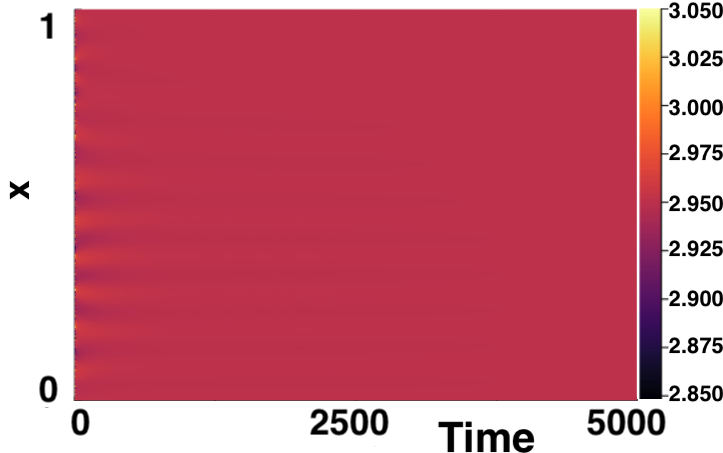
\includegraphics[width=7cm,height=5cm]{p3t05.png}
    \caption{$\tau=0.5$}
    \label{}
\end{subfigure}
\hfill
\begin{subfigure}[t]{0.45\textwidth}
    \centering
    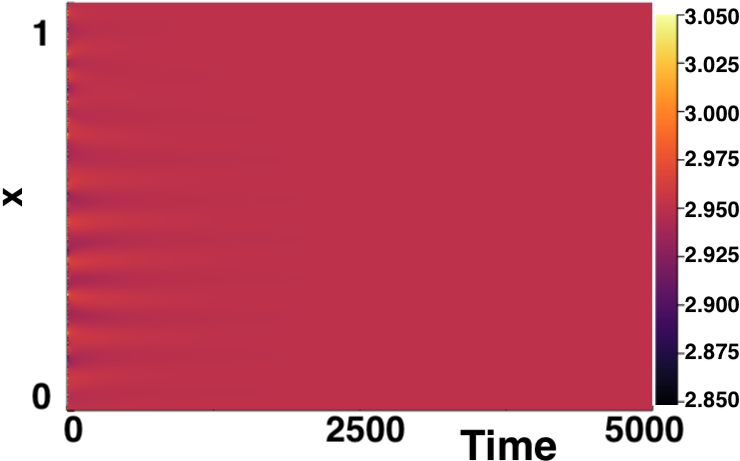
\includegraphics[width=7cm,height=5cm]{p3t1.png}
    \caption{$\tau=1$}
    \label{}
\end{subfigure}
\caption{Numerical simulations of \eqref{fixed2} for $(a,b)=(1.2,1.75)$. $\epsilon^2=0.001$ and $L^2=9/2$. Boundary conditions given by \eqref{neumannbc} and initial conditions by \eqref{firstic}. We see no Turing pattern formation for $\tau\in\{0.5,1\}$ as suggested by linear theory, seen in Figure \ref{fig:tspacetau}. }
\label{fig:appfig1}
\end{figure}
\begin{figure}[H]
  \centering
\begin{subfigure}[t]{0.45\textwidth}
    \centering
    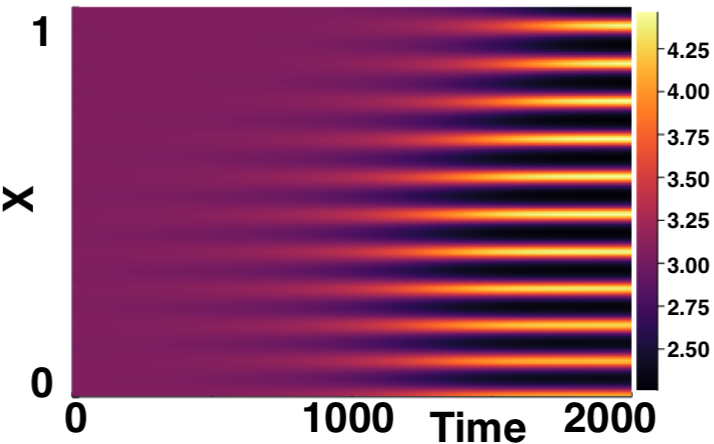
\includegraphics[width=7cm,height=5cm]{p2t05.png}
    \caption{$\tau=0.5$}
    \label{}
\end{subfigure}
\hfill
\begin{subfigure}[t]{0.45\textwidth}
    \centering
    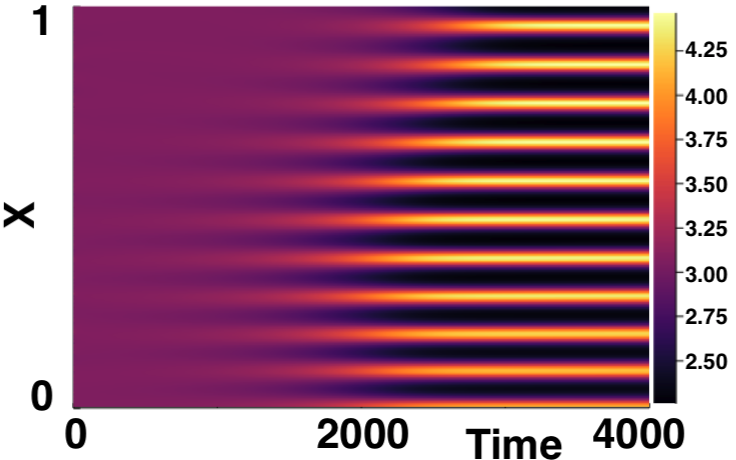
\includegraphics[width=7cm,height=5cm]{p2t1.png}
    \caption{$\tau=1$}
    \label{}
\end{subfigure}
\caption{Numerical simulations of \eqref{fixed2} for $(a,b)=(1.2,1.85)$. $\epsilon^2=0.001$ and $L^2=9/2$. Boundary conditions given by \eqref{neumannbc} and initial conditions by \eqref{firstic}. We see Turing pattern formation on an increasing timescale for $\tau\in\{0.5,1\}$ as suggested by linear theory, seen in Figure \ref{fig:tspacetau}. }
\label{fig:appfig2}
\end{figure}

Figures \ref{fig:Bbif1} and \ref{fig:Bbif2} show analogous bifurcation diagrams to those produced in Figures \ref{fig:lambdavary} and \ref{fig:fixbif2}, with $\tau=0.5,1$.

\begin{figure}[H]
  \centering
\begin{subfigure}[t]{0.45\textwidth}
    \centering
    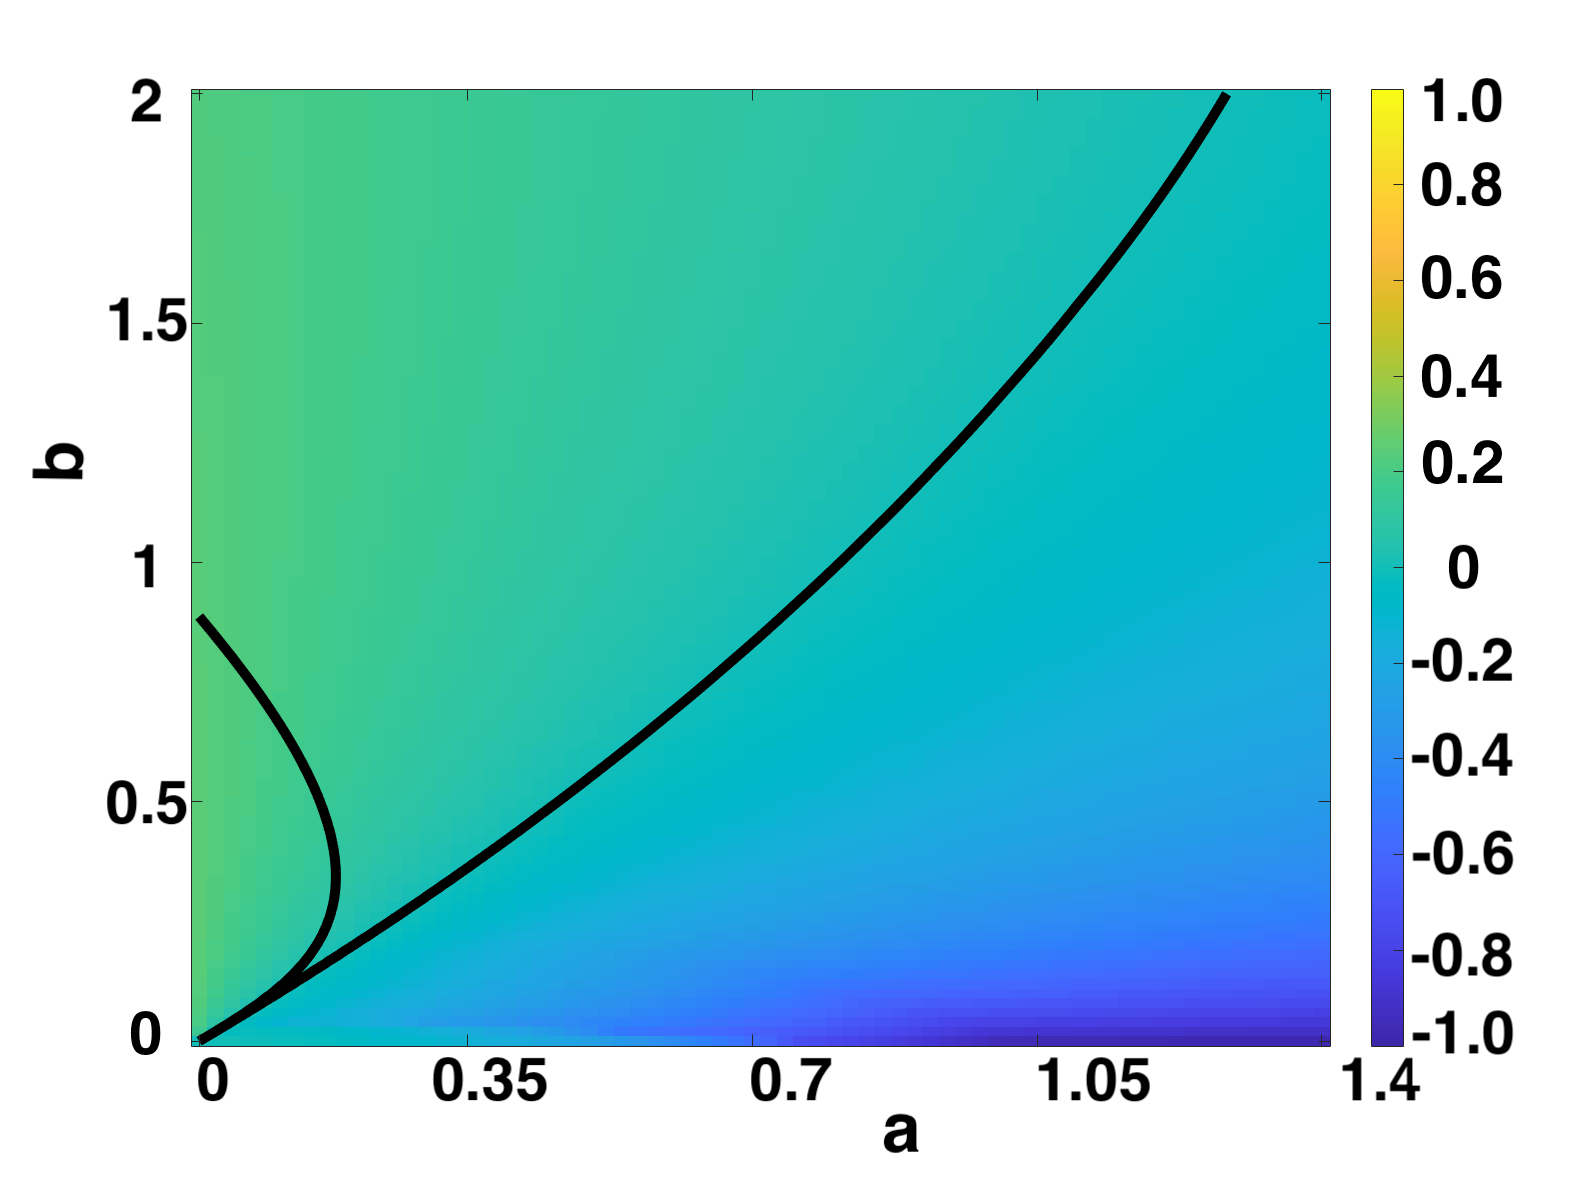
\includegraphics[width=7cm,height=5cm]{tau05bif.png}
    \caption{$\tau=0.5$}
    \label{}
\end{subfigure}
\hfill
\begin{subfigure}[t]{0.45\textwidth}
    \centering
    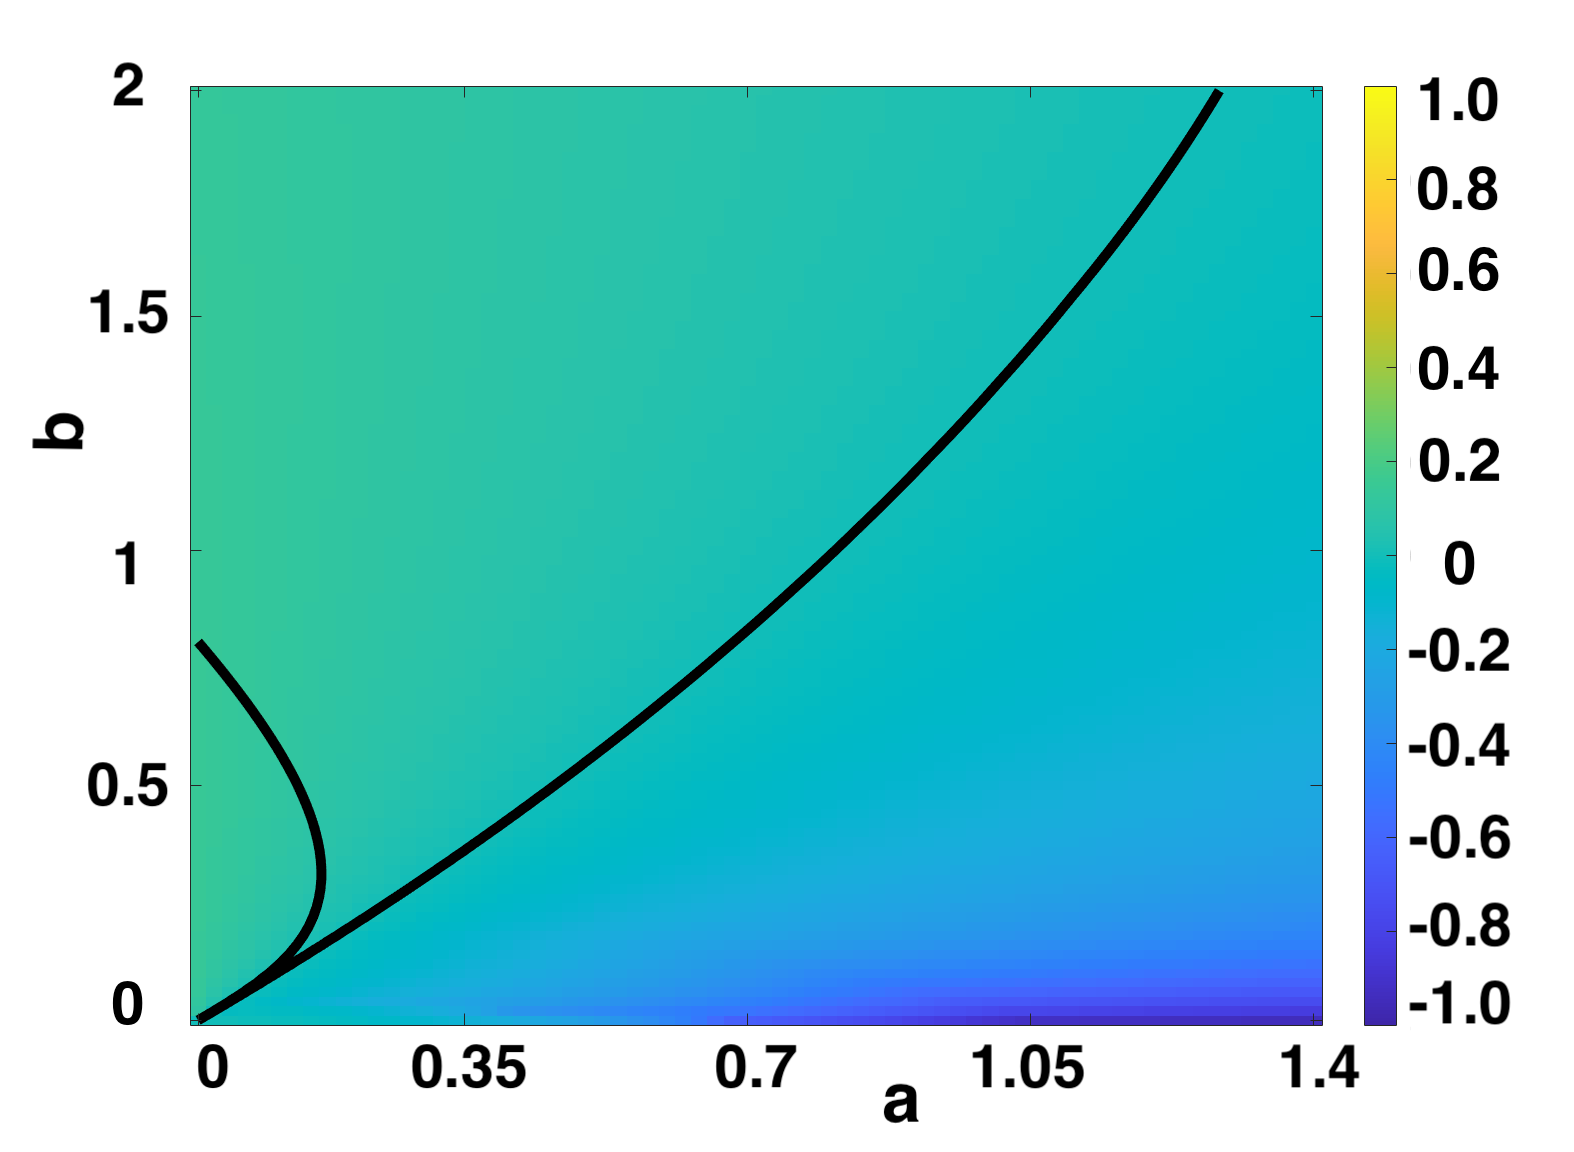
\includegraphics[width=7cm,height=5cm]{tau1bif.png}
    \caption{$\tau=1$}
    \label{}
\end{subfigure}
\caption{$\max_k(\Re(\lambda_k))$ computed over $(a,b)$ parameter space by solving \eqref{realfixbif} and \eqref{complexfixbif}, with $\epsilon^2=0.001$, $L^2=9/2$. As $\tau$ increases, $|\max_k(\Re(\lambda_k))|$ decreases. Contour lines for $\Re(\lambda_0)=0$ and $\max_k(\Re(\lambda_k))=0$ overlayed, indicated Turing instability region. }
\label{fig:Bbif1}
\end{figure}
\begin{figure}[H]
  \centering
\begin{subfigure}[t]{0.45\textwidth}
    \centering
    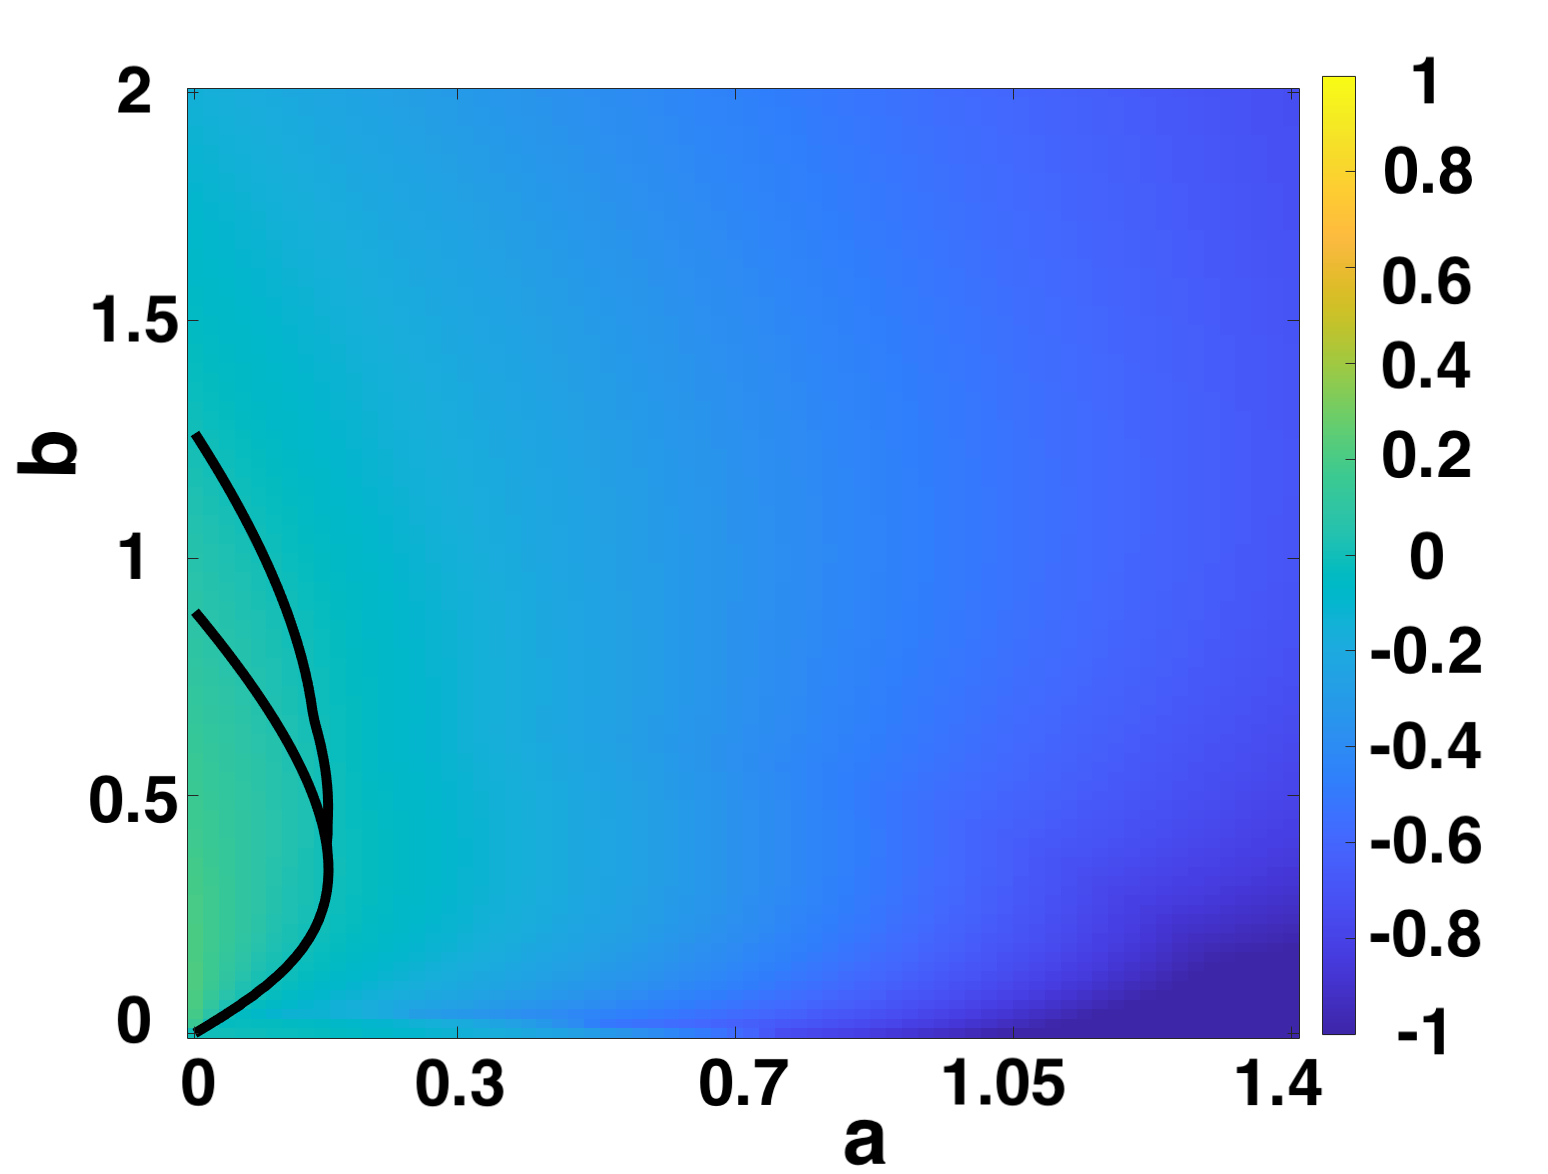
\includegraphics[width=7cm,height=5cm]{fixbif22.png}
    \caption{$\tau=0.5$}
    \label{}
\end{subfigure}
\hfill
\begin{subfigure}[t]{0.45\textwidth}
    \centering
    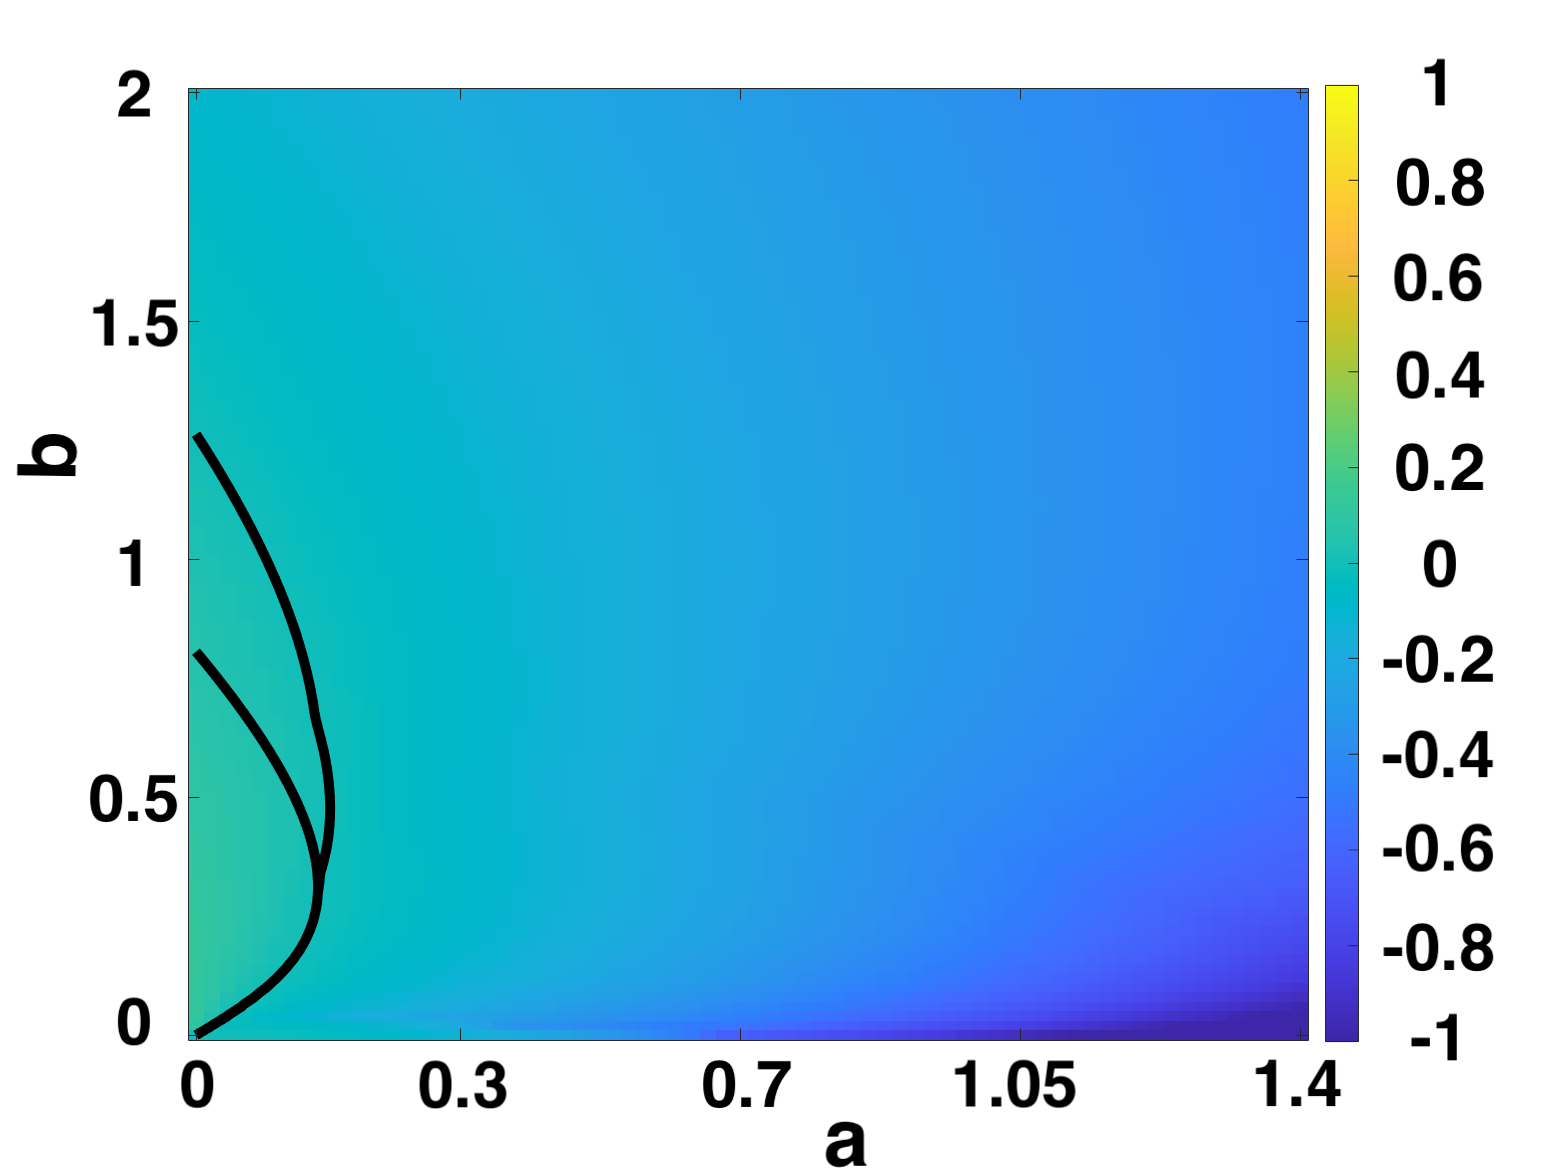
\includegraphics[width=7cm,height=5cm]{fixbif23.png}
    \caption{$\tau=1$}
    \label{}
\end{subfigure}
\caption{$\max_k(\Re(\lambda_k))$ computed over $(a,b)$ parameter space by solving \eqref{realfixbif} and \eqref{complexfixbif}, with $\epsilon^2=0.1$, $L^2=9/2$. As $\tau$ increases, $|\max_k(\Re(\lambda_k))|$ decreases. Contour lines for $\Re(\lambda_0)=0$ and $\max_k(\Re(\lambda_k))=0$ overlayed, indicated Turing instability region. }
\label{fig:Bbif2}
\end{figure}

In Figures \ref{fig:Bbc2}, \ref{fig:Bbc4} and \ref{fig:Bbc8}, we present the comparison of numerical solutions between boundary conditions $BC_1$ and $BC_2$, for $\tau\in\{2,4,8\}$.

\begin{figure}[H]
    \centering
    \begin{subfigure}[t]{0.45\textwidth}
        \centering
        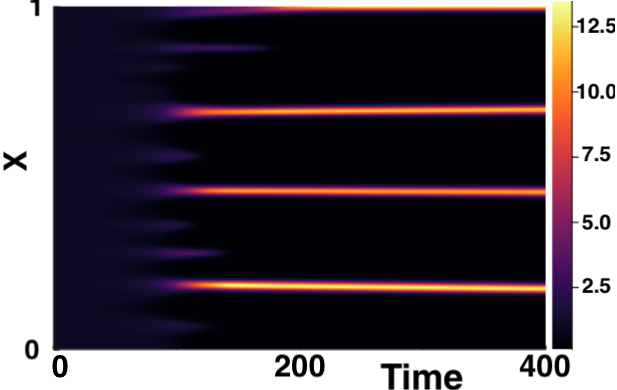
\includegraphics[width=6cm,height=4.5cm]{ic22.png}
        \caption{$\text{BC}_1$ given by equation \eqref{neumannbc}.}
        \label{}
    \end{subfigure}
    \hfill
    \begin{subfigure}[t]{0.45\textwidth}
        \centering
        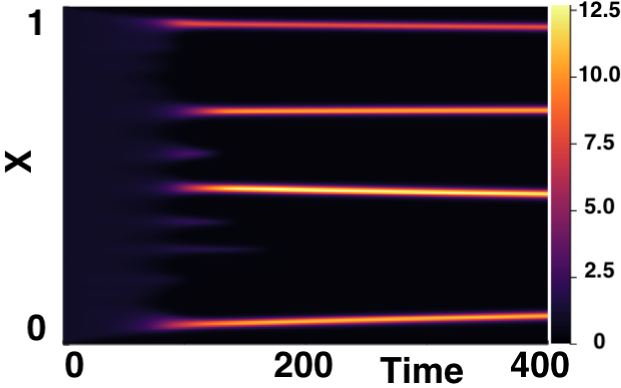
\includegraphics[width=6cm,height=4.5cm]{bc2.png}
        \caption{$\text{BC}_2$ given by equation \eqref{homogeneousbc}.}
        \label{}
    \end{subfigure}
    \caption{Comparison of varying BCs for $\tau=2$. $(a,b)=(0.1,0.9)$, $\epsilon^2=0.001$, $L^2=9/2$. Initial conditions given by \eqref{firstic}.}
    \label{fig:Bbc2}
\end{figure}

\begin{figure}[H]
    \centering
    \begin{subfigure}[t]{0.45\textwidth}
        \centering
        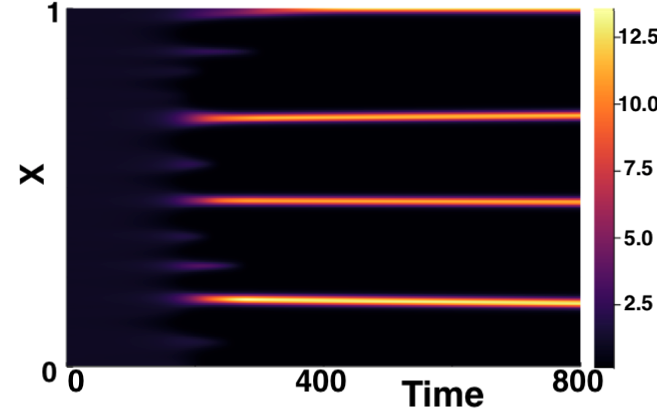
\includegraphics[width=6cm,height=4.5cm]{ic24.png}
        \caption{$\text{BC}_1$ given by equation \eqref{neumannbc}.}
        \label{}
    \end{subfigure}
    \hfill
    \begin{subfigure}[t]{0.45\textwidth}
        \centering
        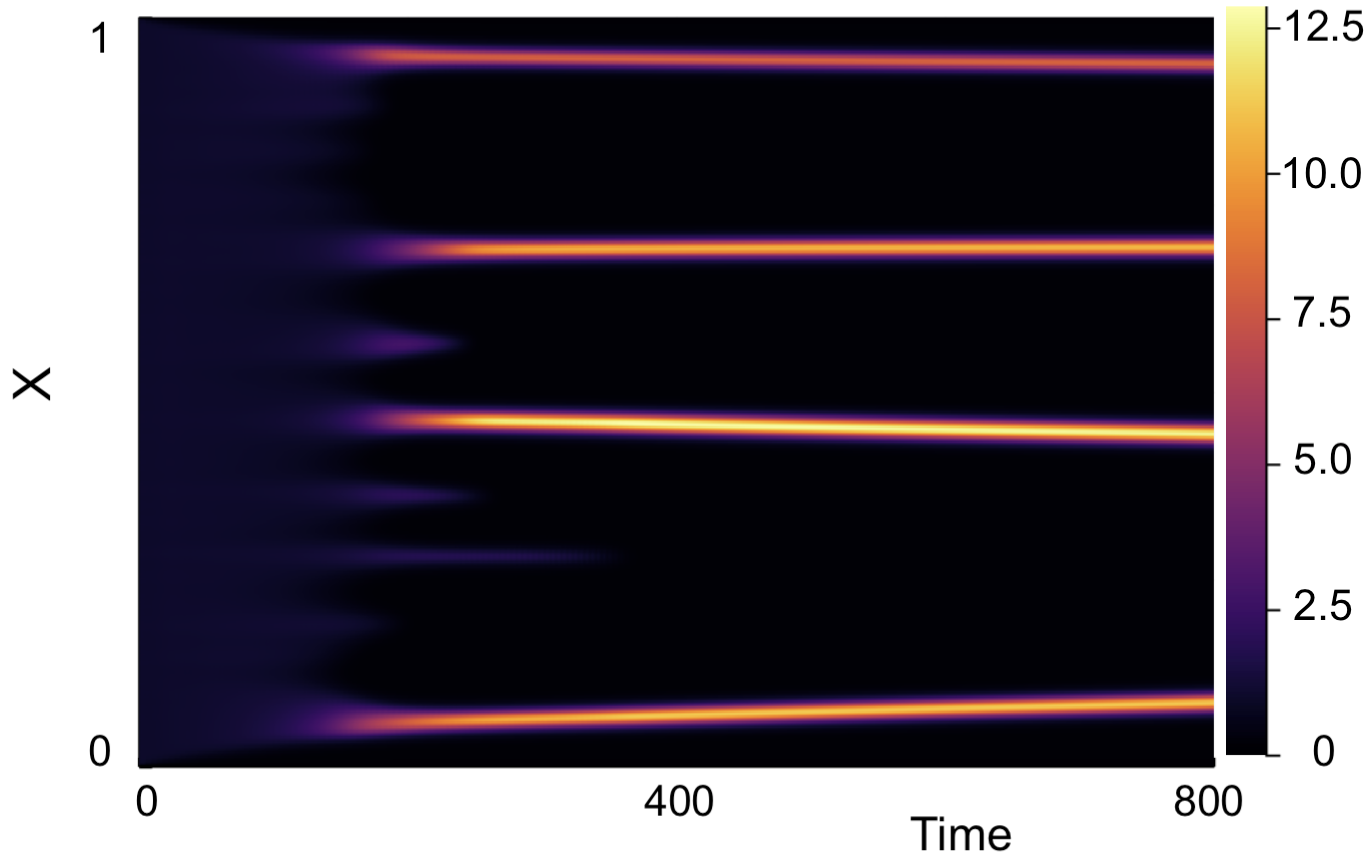
\includegraphics[width=6cm,height=4.5cm]{bc4.png}
        \caption{$\text{BC}_2$ given by equation \eqref{homogeneousbc}.}
        \label{}
    \end{subfigure}
    \caption{Comparison of varying BCs for $\tau=4$. $(a,b)=(0.1,0.9)$, $\epsilon^2=0.001$, $L^2=9/2$. Initial conditions given by \eqref{firstic}.}
    \label{fig:Bbc4}
\end{figure}

\begin{figure}[H]
    \centering
    \begin{subfigure}[t]{0.45\textwidth}
        \centering
        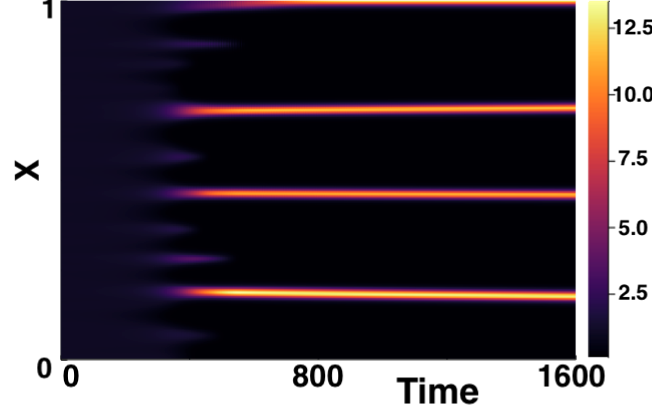
\includegraphics[width=6cm,height=4.5cm]{ic28.png}
        \caption{$\text{BC}_1$ given by equation \eqref{neumannbc}.}
        \label{}
    \end{subfigure}
    \hfill
    \begin{subfigure}[t]{0.45\textwidth}
        \centering
        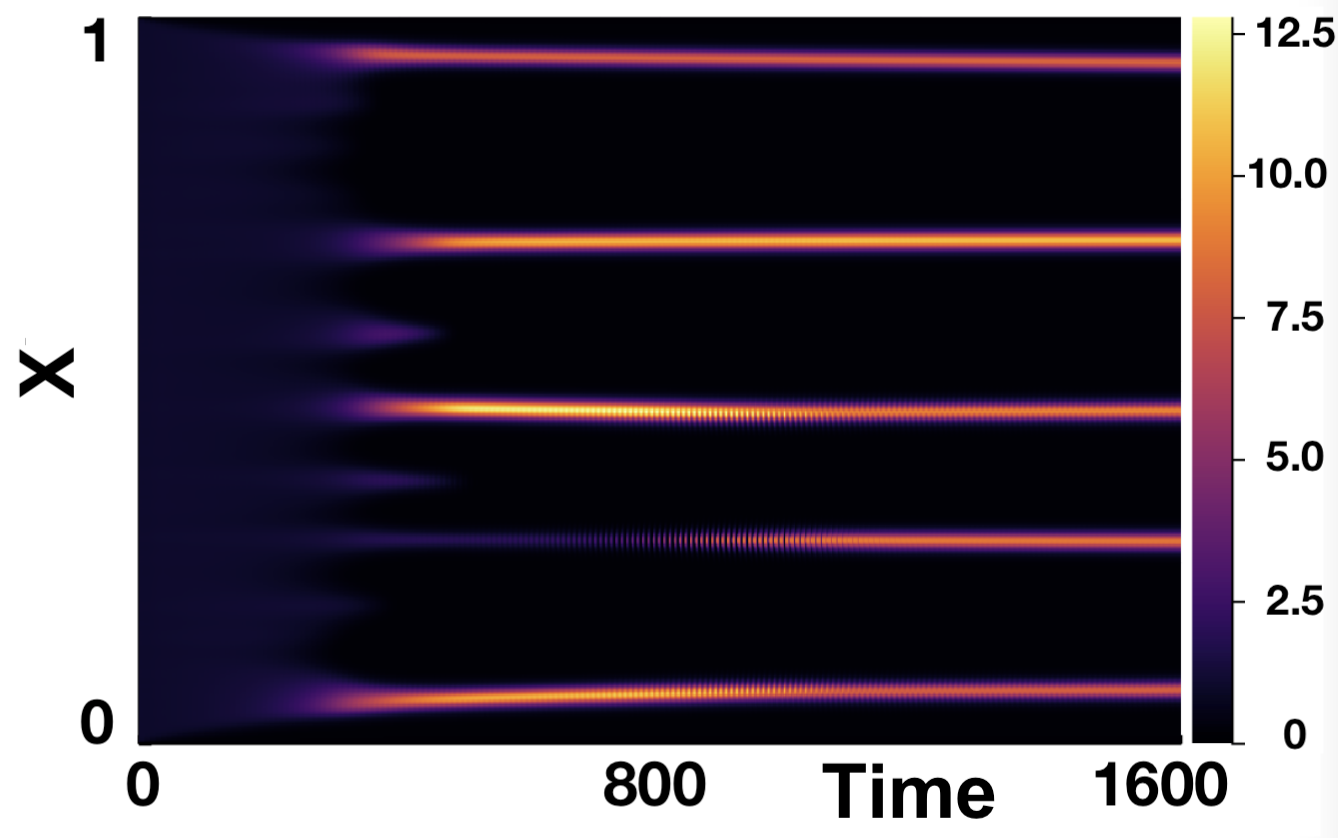
\includegraphics[width=6cm,height=4.5cm]{bc8.png}
        \caption{$\text{BC}_2$ given by equation \eqref{homogeneousbc}.}
        \label{}
    \end{subfigure}
    \caption{Comparison of varying BCs for $\tau=8$. $(a,b)=(0.1,0.9)$, $\epsilon^2=0.001$, $L^2=9/2$. Initial conditions given by \eqref{firstic}.}
    \label{fig:Bbc8}
\end{figure}

In Figures \ref{fig:temp1}, \ref{fig:temp2}, \ref{fig:temp4}, \ref{fig:temp8} and \ref{fig:temp16} show the preliminary results for a temporal variation in the history function on the time-to-pattern properties. We consider two history functions, namely $h(t)=u_\star(1+r\sin(\omega t))$, for $\omega=1/7,4/7$ for $t\in[-\tau,0)$, where $r$ is the random variable used in $\text{IC}_2$. The history functions with $\omega=1/7,4/7$ will be denoted $h_1(t)$, and $h_2(t)$ repectively. For each $\tau\in\{1,2,4,8,16\}$, we compare the results for each of these variations in history function with the numerical results simulated with the history function equal to the initial conditions, as given in \eqref{hist}. We see that these variations in the history function do not signficantly effect the timescales on which pattern formation occurs.

\begin{figure}[H]
    \centering
    \begin{subfigure}[t]{0.32\textwidth}
        \centering
        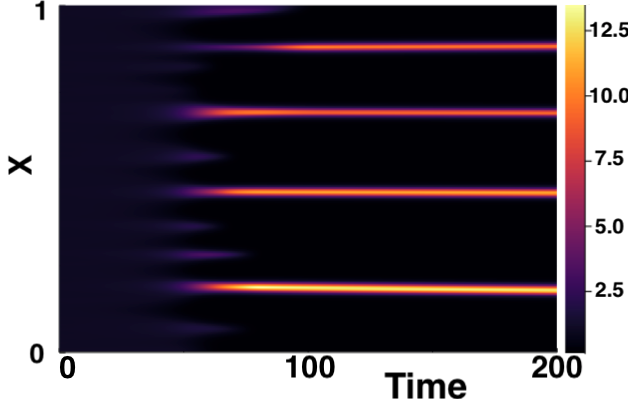
\includegraphics[width=5cm,height=4.5cm]{ic21.png}
        \caption{History function given as in \eqref{hist}.}
        \label{}
    \end{subfigure}
    \hfill
    \begin{subfigure}[t]{0.32\textwidth}
        \centering
        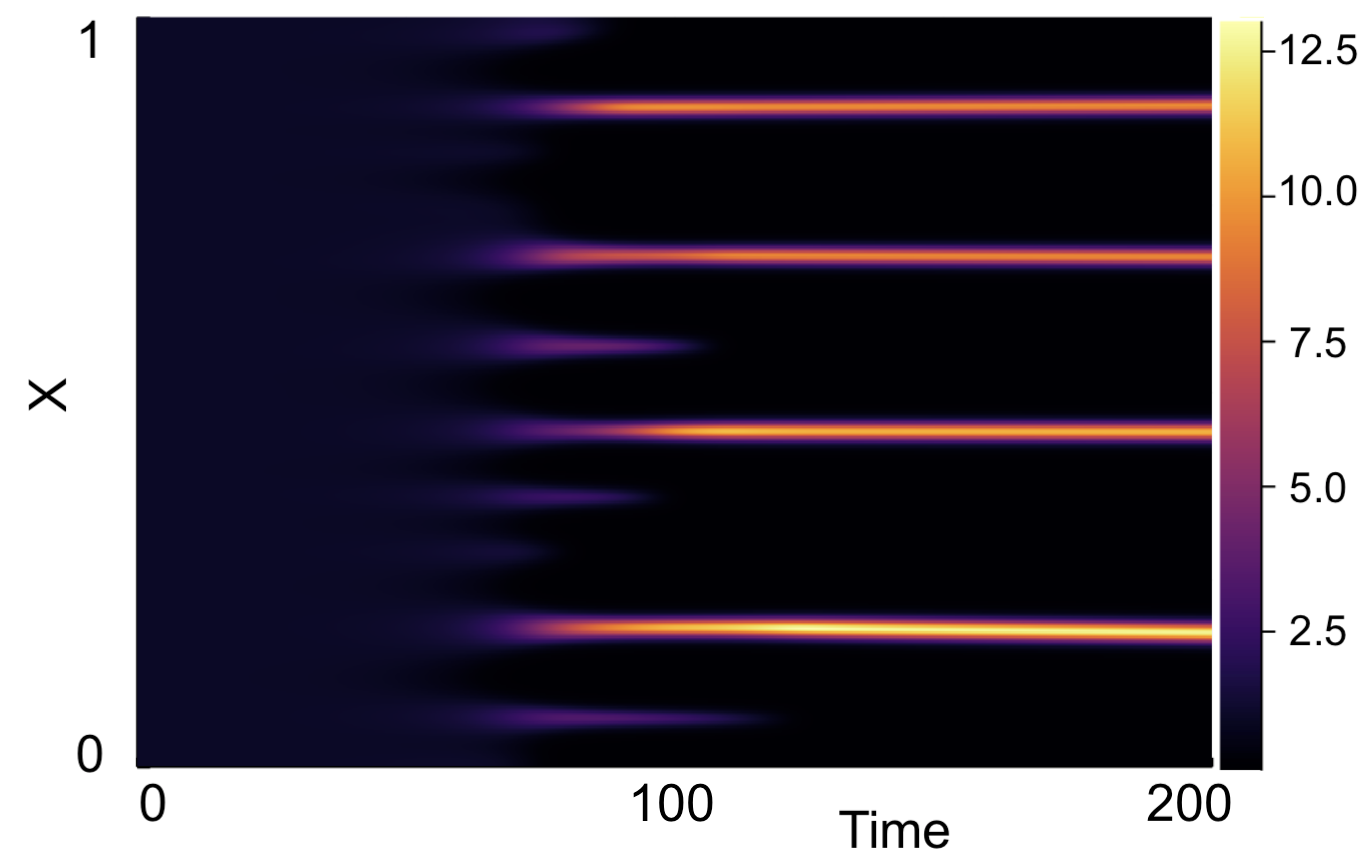
\includegraphics[width=5cm,height=4.5cm]{h11.png}
        \caption{History function $h_1(t)$.}
        \label{}
    \end{subfigure}
    \hfill
    \begin{subfigure}[t]{0.32\textwidth}
        \centering
        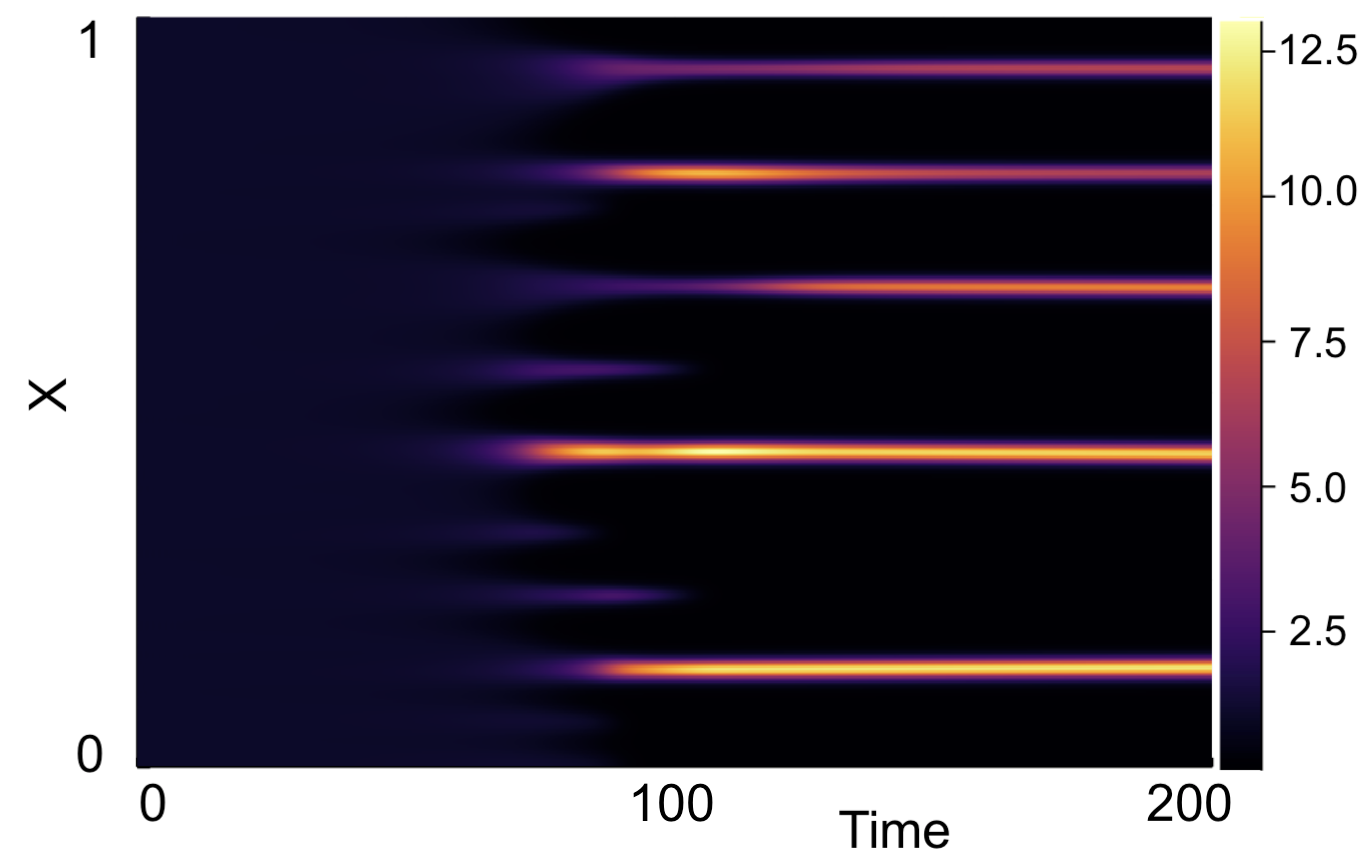
\includegraphics[width=5cm,height=4.5cm]{h21.png}
        \caption{History function $h_2(t)$.}
        \label{}
    \end{subfigure}
    \caption{Numerical simulations of \eqref{fixed2} showing comparison of varying history functions for $\tau=1$. Boundary conditions given by \eqref{neumannbc} and initial conditions by \eqref{firstic}. Parameters $(a,b)=(0.1,0.9)$, $\epsilon^2=0.001$, $L^2=9/2$ used.}
    \label{fig:temp1}
\end{figure}
\begin{figure}[H]
    \centering
    \begin{subfigure}[t]{0.32\textwidth}
        \centering
        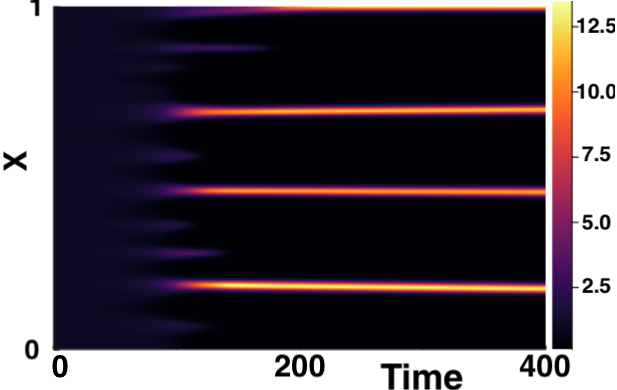
\includegraphics[width=5cm,height=4.5cm]{ic22.png}
        \caption{History function given as in \eqref{hist}.}
        \label{}
    \end{subfigure}
    \hfill
    \begin{subfigure}[t]{0.32\textwidth}
        \centering
        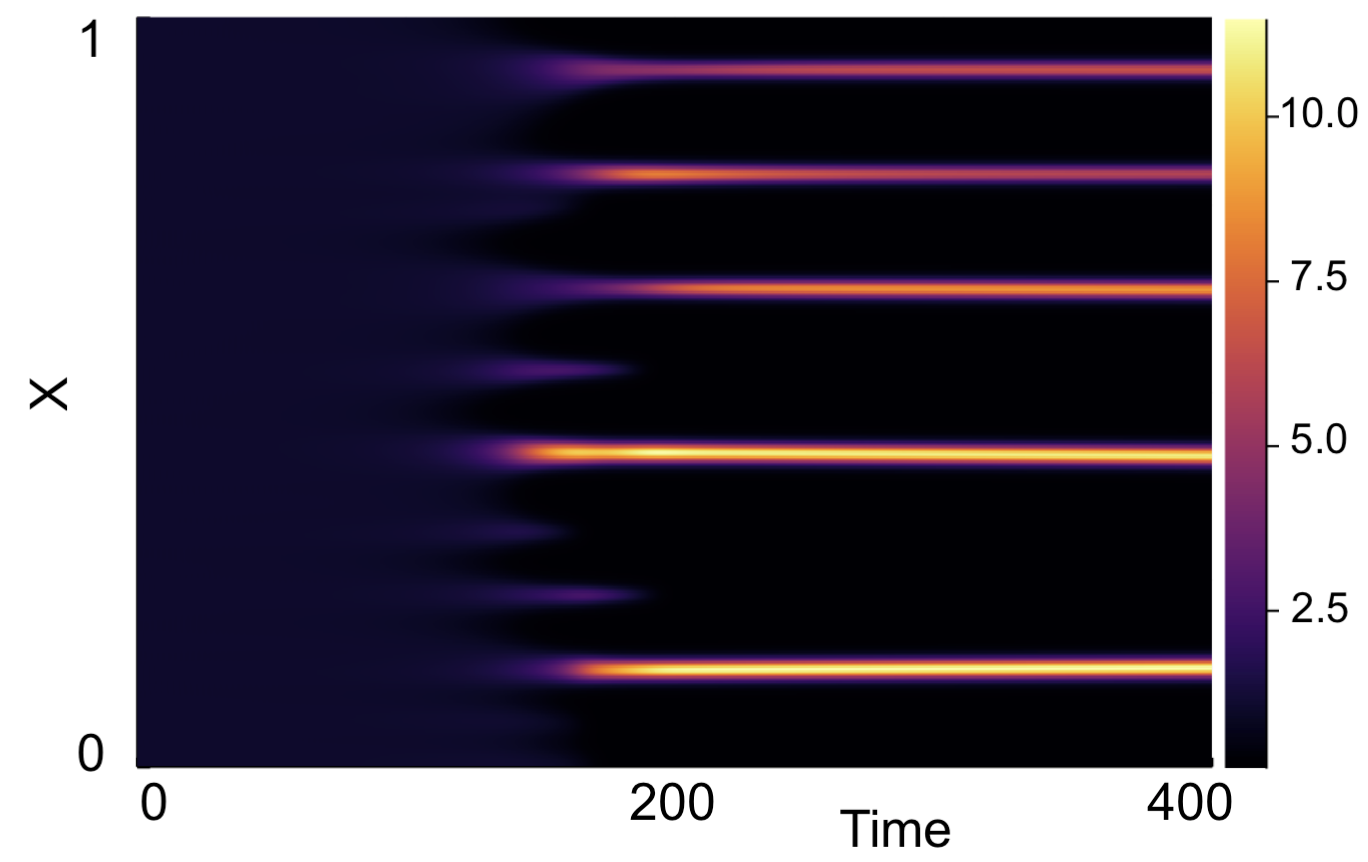
\includegraphics[width=5cm,height=4.5cm]{h12.png}
        \caption{History function $h_1(t)$.}
        \label{}
    \end{subfigure}
    \hfill
    \begin{subfigure}[t]{0.32\textwidth}
        \centering
        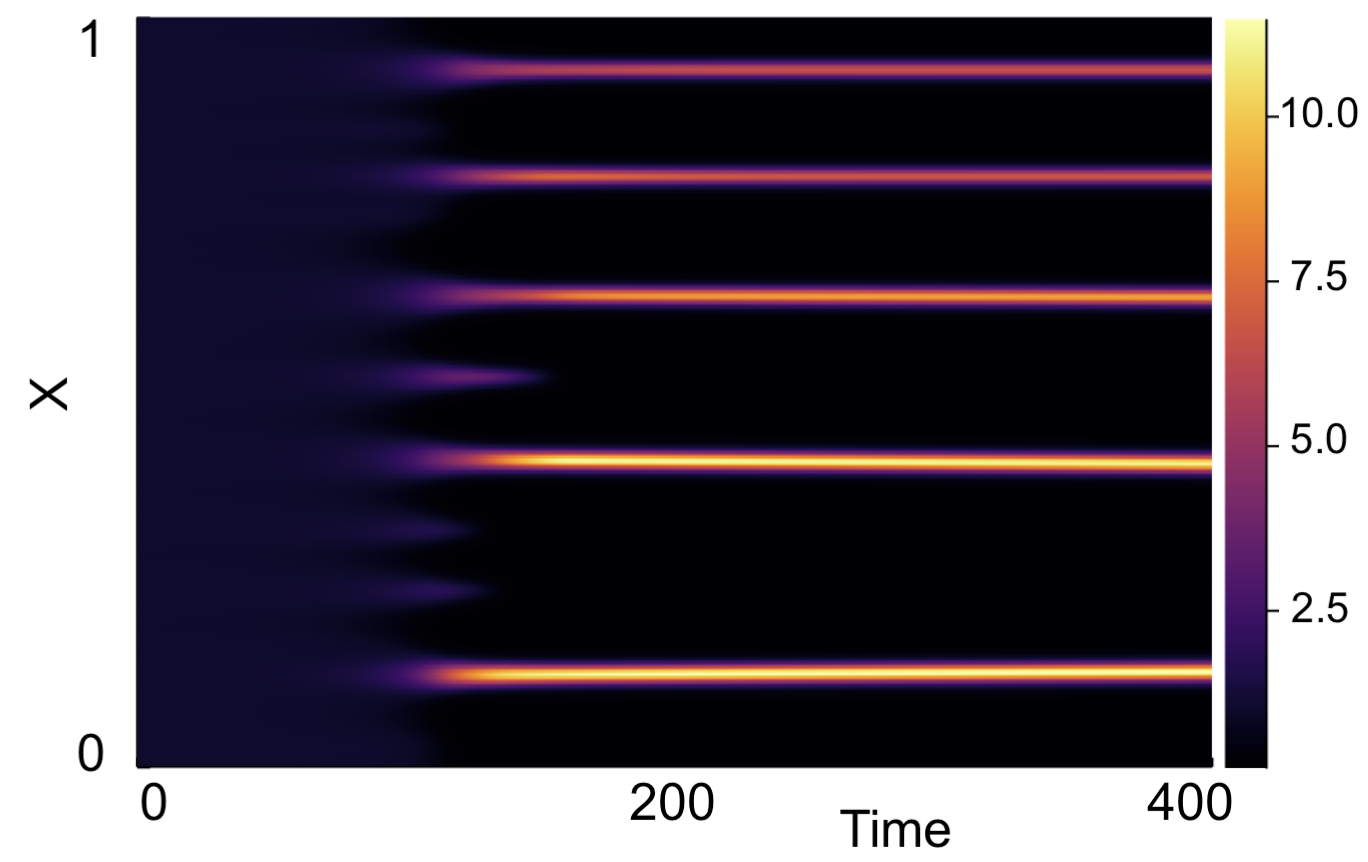
\includegraphics[width=5cm,height=4.5cm]{h22.png}
        \caption{History function $h_2(t)$.}
        \label{}
    \end{subfigure}
    \caption{Numerical simulations of \eqref{fixed2} showing comparison of varying history functions for $\tau=2$. Boundary conditions given by \eqref{neumannbc} and initial conditions by \eqref{firstic}. Parameters $(a,b)=(0.1,0.9)$, $\epsilon^2=0.001$, $L^2=9/2$ used.}
    \label{fig:temp2}
\end{figure}
\begin{figure}[H]
    \centering
    \begin{subfigure}[t]{0.32\textwidth}
        \centering
        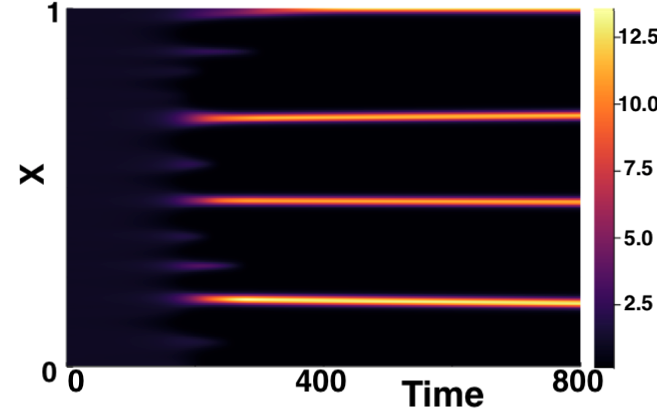
\includegraphics[width=5cm,height=4.5cm]{ic24.png}
        \caption{History function given as in \eqref{hist}.}
        \label{}
    \end{subfigure}
    \hfill
    \begin{subfigure}[t]{0.32\textwidth}
        \centering
        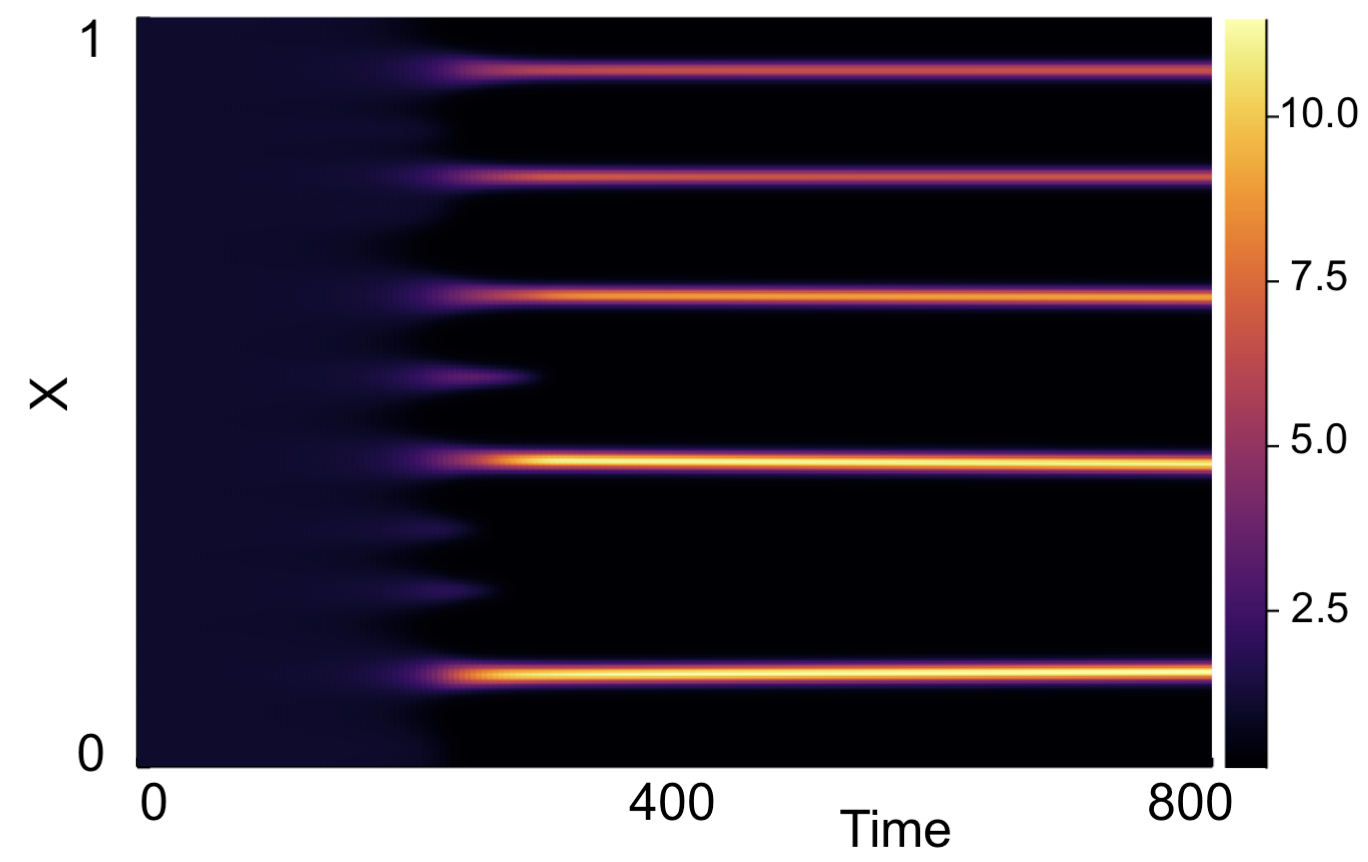
\includegraphics[width=5cm,height=4.5cm]{h14.png}
        \caption{History function $h_1(t)$.}
        \label{}
    \end{subfigure}
    \hfill
    \begin{subfigure}[t]{0.32\textwidth}
        \centering
        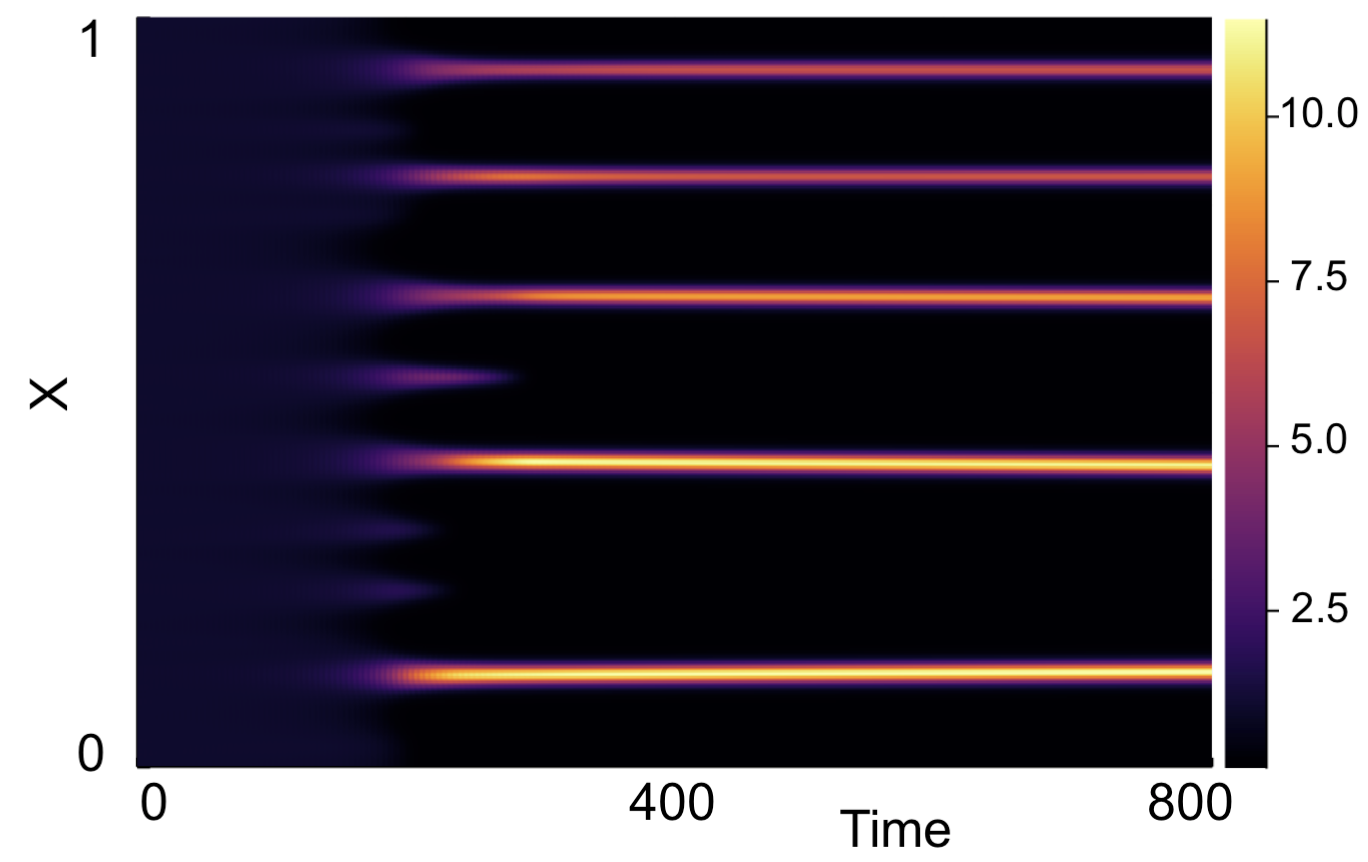
\includegraphics[width=5cm,height=4.5cm]{h24.png}
        \caption{History function $h_2(t)$.}
        \label{}
    \end{subfigure}
    \caption{Numerical simulations of \eqref{fixed2} showing comparison of varying history functions for $\tau=4$. Boundary conditions given by \eqref{neumannbc} and initial conditions by \eqref{firstic}. Parameters $(a,b)=(0.1,0.9)$, $\epsilon^2=0.001$, $L^2=9/2$ used.}
    \label{fig:temp4}
\end{figure}
\begin{figure}[H]
    \centering
    \begin{subfigure}[t]{0.32\textwidth}
        \centering
        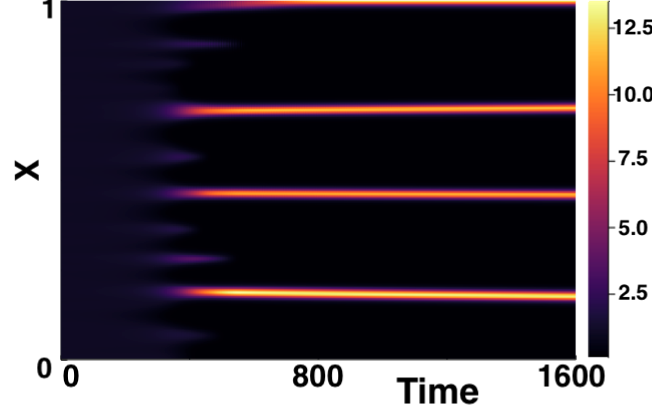
\includegraphics[width=5cm,height=4.5cm]{ic28.png}
        \caption{History function given as in \eqref{hist}.}
        \label{}
    \end{subfigure}
    \hfill
    \begin{subfigure}[t]{0.32\textwidth}
        \centering
        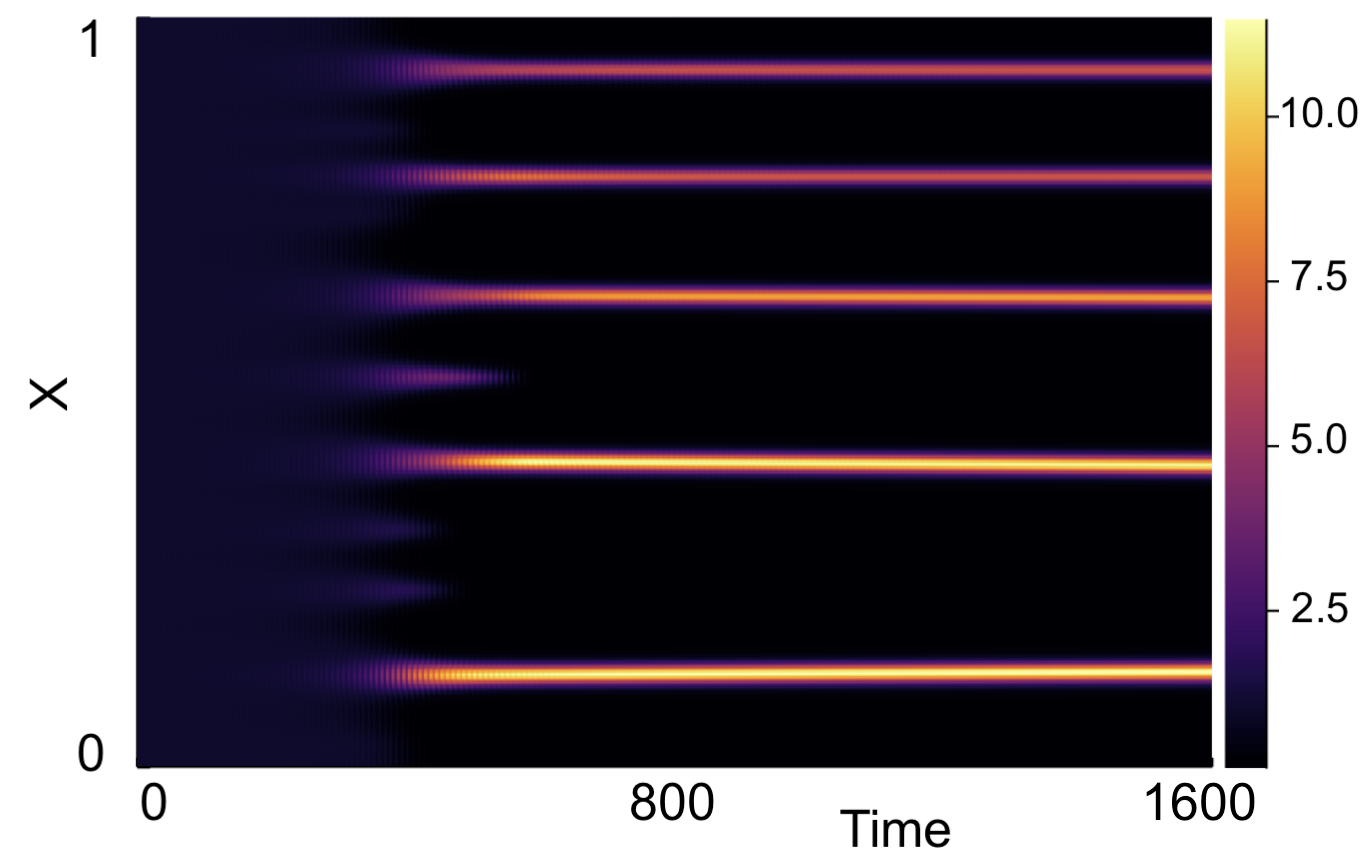
\includegraphics[width=5cm,height=4.5cm]{h18.png}
        \caption{History function $h_1(t)$.}
        \label{}
    \end{subfigure}
    \hfill
    \begin{subfigure}[t]{0.32\textwidth}
        \centering
        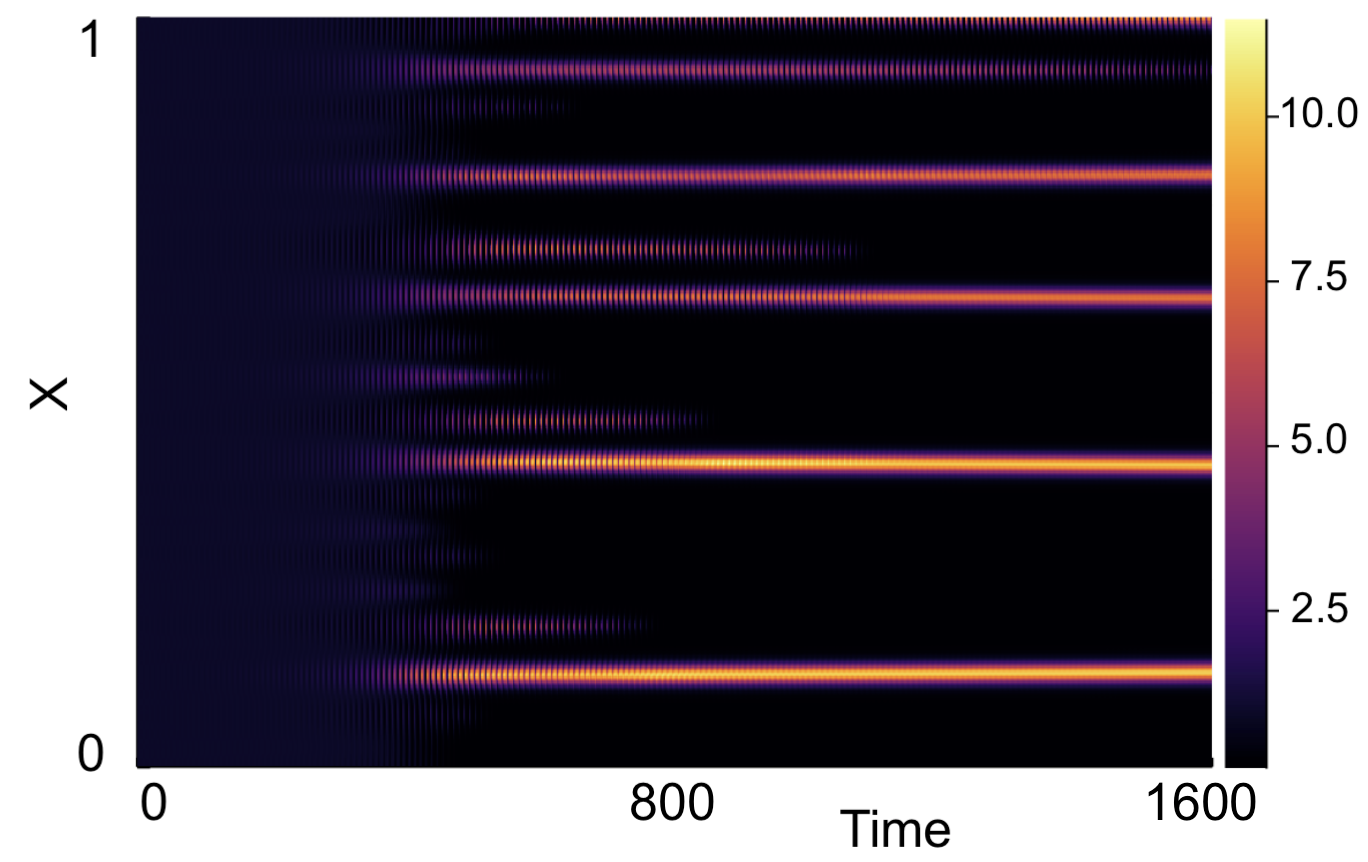
\includegraphics[width=5cm,height=4.5cm]{h28.png}
        \caption{History function $h_2(t)$.}
        \label{}
    \end{subfigure}
    \caption{Numerical simulations of \eqref{fixed2} showing comparison of varying history functions for $\tau=8$. Boundary conditions given by \eqref{neumannbc} and initial conditions by \eqref{firstic}. Parameters $(a,b)=(0.1,0.9)$, $\epsilon^2=0.001$, $L^2=9/2$ used.}
    \label{fig:temp8}
\end{figure}
\begin{figure}[H]
    \centering
    \begin{subfigure}[t]{0.32\textwidth}
        \centering
        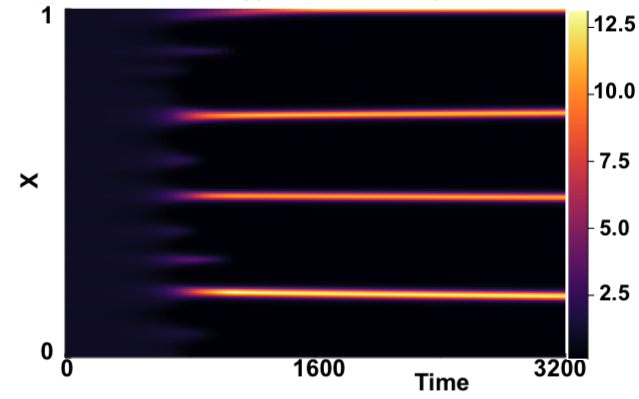
\includegraphics[width=5cm,height=4.5cm]{ic216.png}
        \caption{History function given as in \eqref{hist}.}
        \label{}
    \end{subfigure}
    \hfill
    \begin{subfigure}[t]{0.32\textwidth}
        \centering
        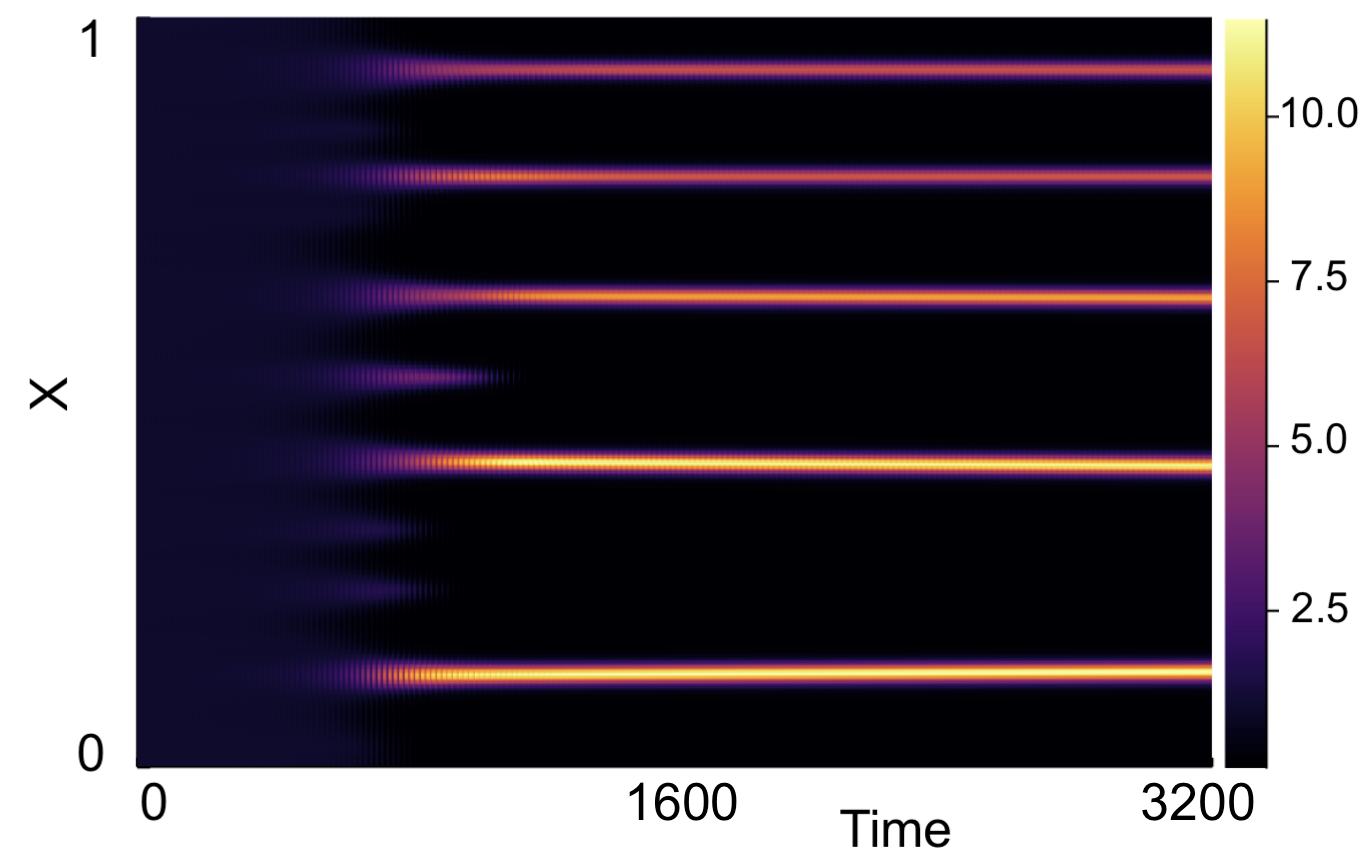
\includegraphics[width=5cm,height=4.5cm]{h116.png}
        \caption{History function $h_1(t)$.}
        \label{}
    \end{subfigure}
    \hfill
    \begin{subfigure}[t]{0.32\textwidth}
        \centering
        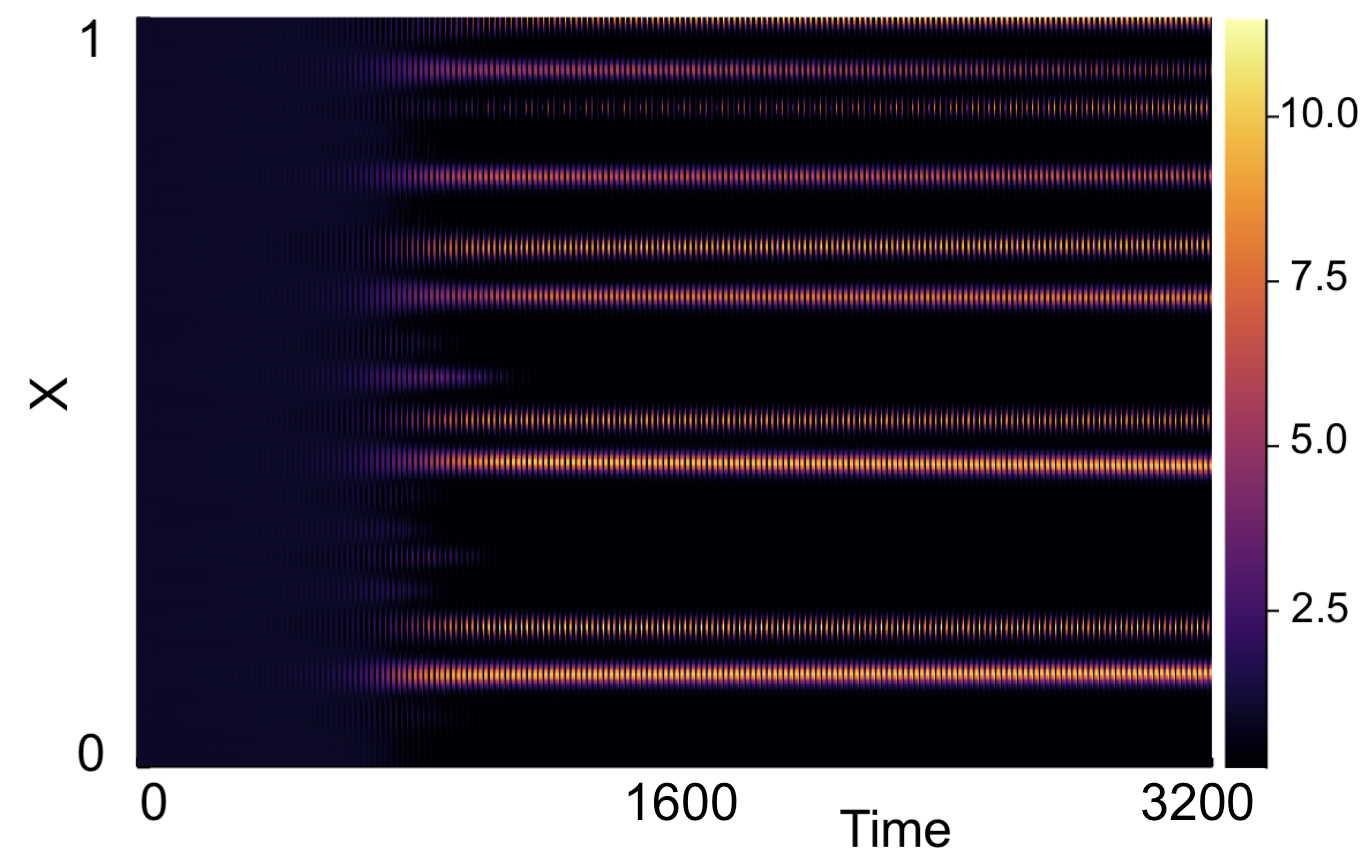
\includegraphics[width=5cm,height=4.5cm]{h216.png}
        \caption{History function $h_2(t)$.}
        \label{}
    \end{subfigure}
    \caption{Numerical simulations of \eqref{fixed2} showing comparison of varying history functions for $\tau=16$. Boundary conditions given by \eqref{neumannbc} and initial conditions by \eqref{firstic}. Parameters $(a,b)=(0.1,0.9)$, $\epsilon^2=0.001$, $L^2=9/2$ used.}
    \label{fig:temp16}
\end{figure}

In Figure \ref{fig:Bbif4}, we present results showing a linear relationship between time delay and time-to-pattern for the same parameter values used in Figure \ref{fig:linperturb1}, but with a threshold value $2$, from a $\sigma_{\text{IC}}=0.01$.

\begin{figure}[H]
   \centering
   \begin{subfigure}[t]{0.45\textwidth}
       \centering
       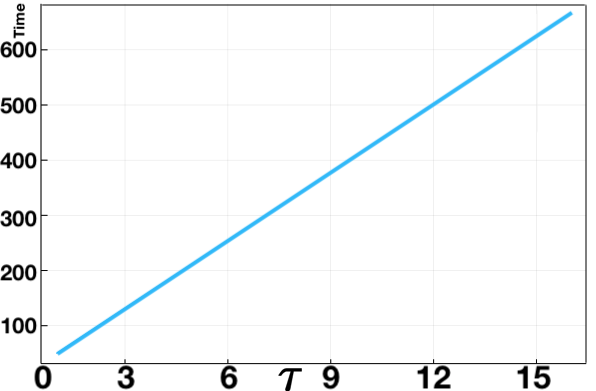
\includegraphics[width=7cm,height=5cm]{longlin1.png}
       \caption{$(a,b)=(0.1,0.9)$}
       \label{}
   \end{subfigure}
   \hfill
   \begin{subfigure}[t]{0.45\textwidth}
       \centering
       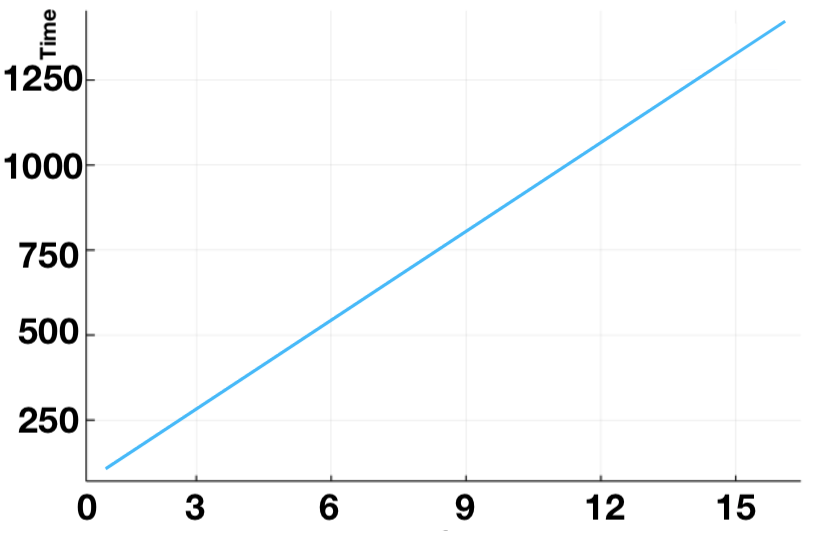
\includegraphics[width=7cm,height=5cm]{longlin4.png}
       \caption{$(a,b)=(0.4,0.8)$}
       \label{}
   \end{subfigure}
   \caption{Time-to-pattern for full numerical solutions of \eqref{fixed2} plotted against $\tau\in[1,16]$ for $\sigma_{\text{IC}}=0.01$ and threshold $2$. Parameters used are $\epsilon^2=0.001$ and domain size $L^2=9/2$.}
   \label{fig:Bbif4}
\end{figure}


\section{For Chapter 3}\label{section:Bdist}
\subsection{A Symmetric Distribution}
We present results for the composite Simpson's rule to motivate a choice of $N=50$ temporal discretisation points. Figure \ref{fig:quad} shows the relative error for $N\in[10,200]$ varied at regular intervals of $10$, for the quadrature rule applied to the symmetric truncated Gaussian pdf $k(s;\tau,\sigma)$. We vary $\tau\in\{1,8,16\}$, and for each $\tau$ consider $\sigma\in\{\sigma_{\max}\times0.99,\sigma_{\max}\times0.2,\sigma_{\max}\times0.1\}$. Figure \ref{fig:tempquad} shows the relative error across both the spatial and temporal domains for the quadrature rule applied to the test integral, given in \eqref{testint}, for a the same varying $\tau$, and $\sigma=\sigma_{\max}\times0.99$. Results are shown here for only one $\sigma$ value, as it was found that the relative error was the same, independent of the $\sigma$ used.

\begin{figure}[H]
    \centering
    \begin{subfigure}[t]{0.32\textwidth}
        \centering
        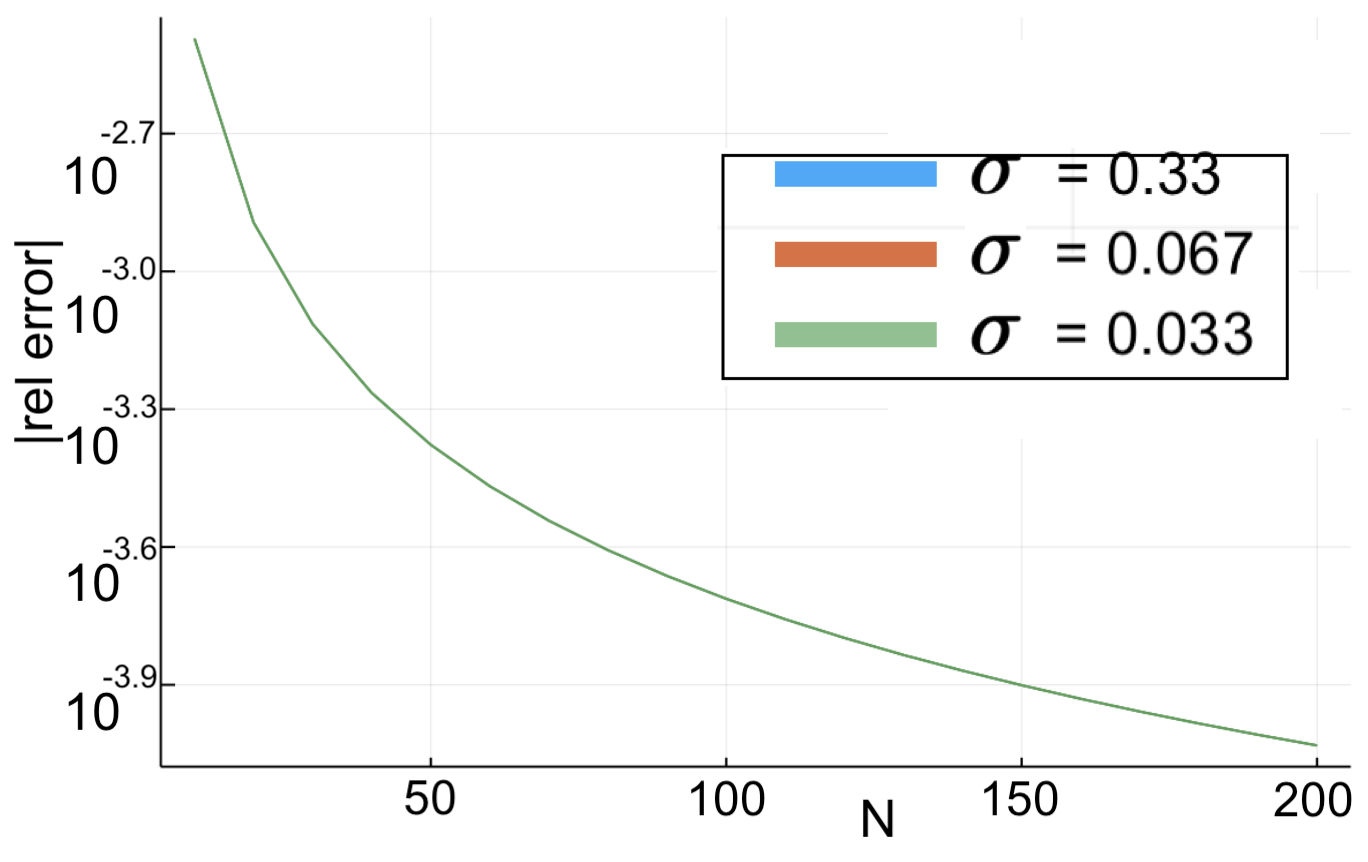
\includegraphics[width=5cm,height=4.5cm]{quadt1.png}
        \caption{$\tau=1$.}
        \label{}
    \end{subfigure}
    \hfill
    \begin{subfigure}[t]{0.32\textwidth}
        \centering
        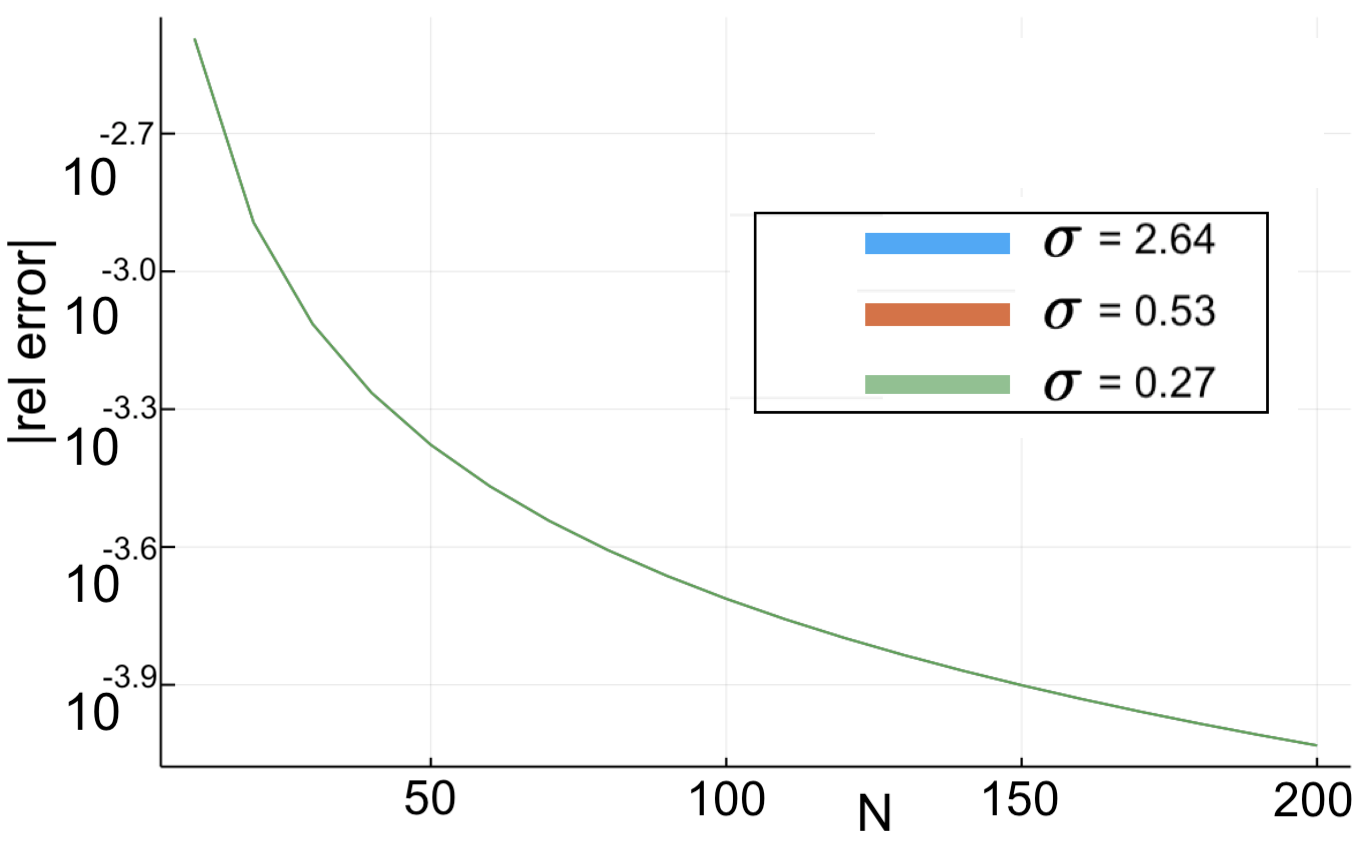
\includegraphics[width=5cm,height=4.5cm]{quadt8.png}
        \caption{$\tau=8$.}
        \label{}
    \end{subfigure}
    \hfill
    \begin{subfigure}[t]{0.32\textwidth}
        \centering
        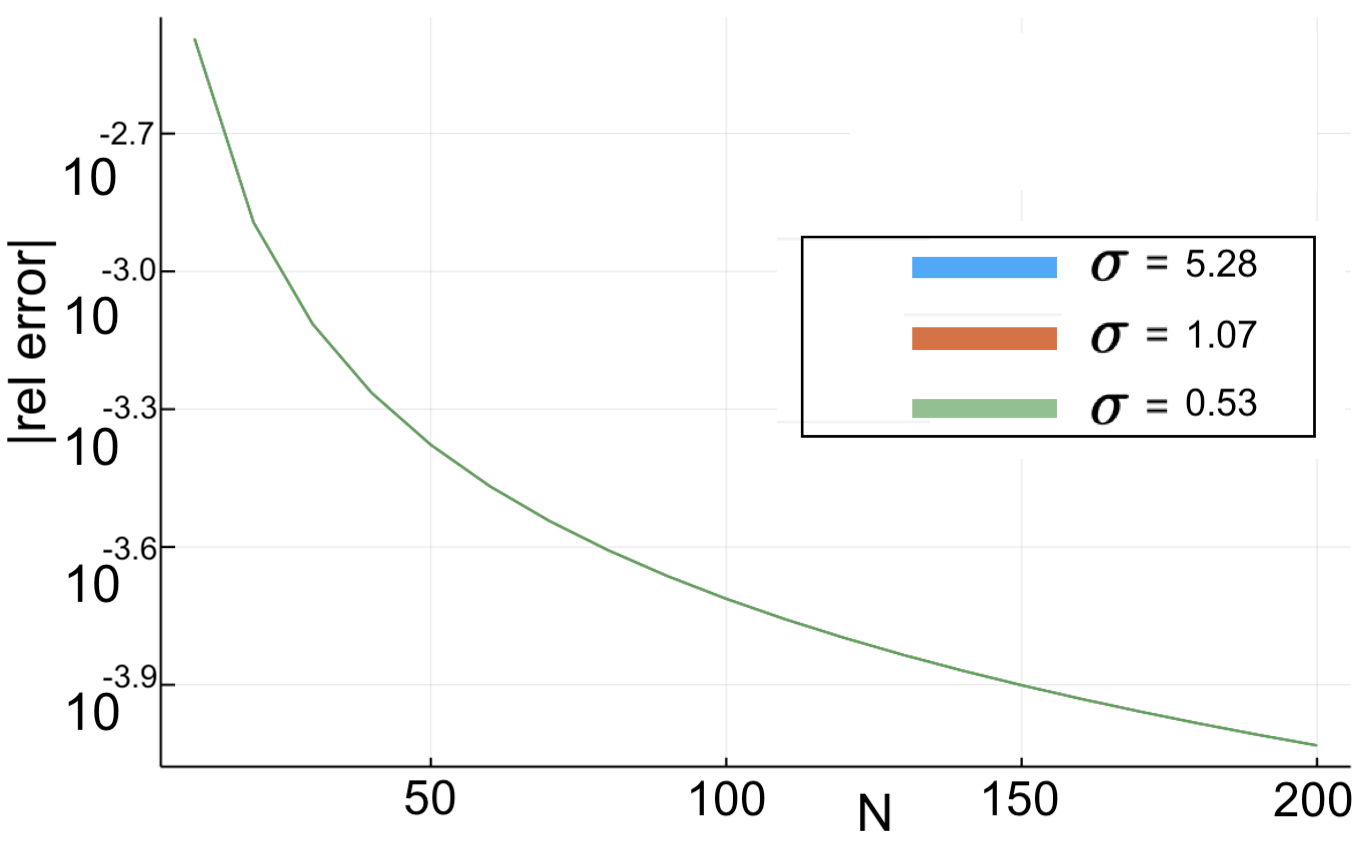
\includegraphics[width=5cm,height=4.5cm]{quadt16.png}
        \caption{$\tau=16$.}
        \label{}
    \end{subfigure}
    \caption{Relative error of composite Simpson's rule applied to integrating $k(s;\tau,\sigma)$ for varying $\tau\in\{1,8,16\}$ and $\sigma\in\{\sigma_{\max}\times0.99,\sigma_{\max}\times0.2,\sigma_{\max}\times0.1\}$. Number of discretisation points varied $N\in[10,200]$ at regular intervals of $10$.}
    \label{fig:quad}
\end{figure}

\begin{figure}[H]
    \centering
    \begin{subfigure}[t]{0.32\textwidth}
        \centering
        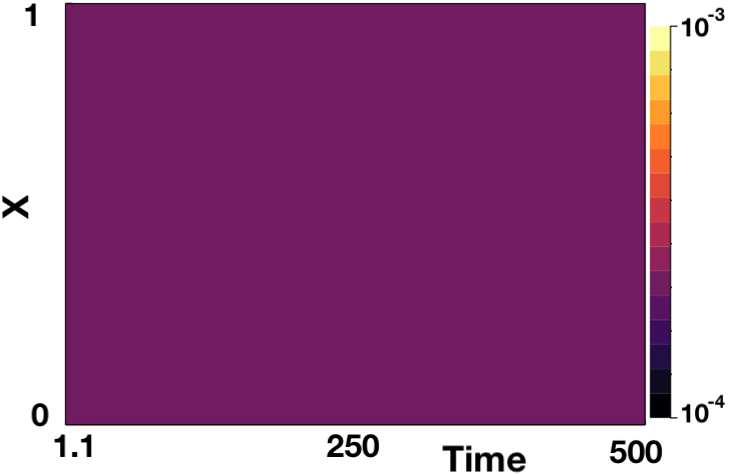
\includegraphics[width=5cm,height=4.5cm]{disterr.png}
        \caption{$\tau=1$.}
        \label{}
    \end{subfigure}
    \hfill
    \begin{subfigure}[t]{0.32\textwidth}
        \centering
        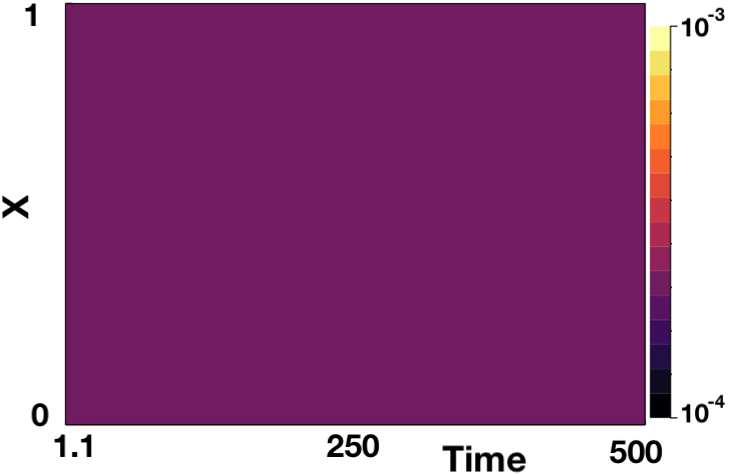
\includegraphics[width=5cm,height=4.5cm]{disterr.png}
        \caption{$\tau=8$.}
        \label{}
    \end{subfigure}
    \hfill
    \begin{subfigure}[t]{0.32\textwidth}
        \centering
        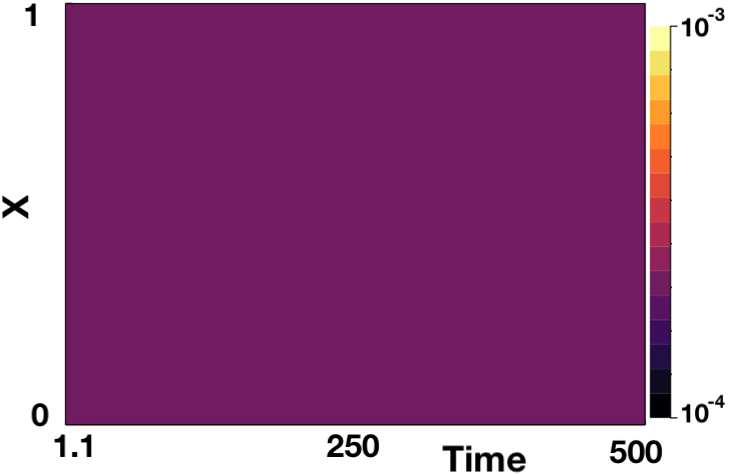
\includegraphics[width=5cm,height=4.5cm]{disterr.png}
        \caption{$\tau=16$.}
        \label{}
    \end{subfigure}
    \caption{Relative error of composite Simpson's rule applied to integrating test integral given in \eqref{testint} for varying $\tau\in\{1,8,16\}$, and $\sigma=\sigma_{\max}\times0.1\}$. $N=50$ discresised at regular intervals of $10$.}
    \label{fig:tempquad}
\end{figure}

In Figures \ref{fig:distheat1} and \ref{fig:distheat2}, we show the fixed delay bifurcation diagrams for varying $\tau$ values for $\epsilon^2=0.001$. Figures \ref{fig:distmap1} and \ref{fig:distmap2} show the distributed delay bifurcation diagrams for varying $\sigma$, for selected $\tau$ and $\epsilon^2$.
\begin{figure}[H]
    \centering
    \begin{subfigure}[t]{0.45\textwidth}
        \centering
        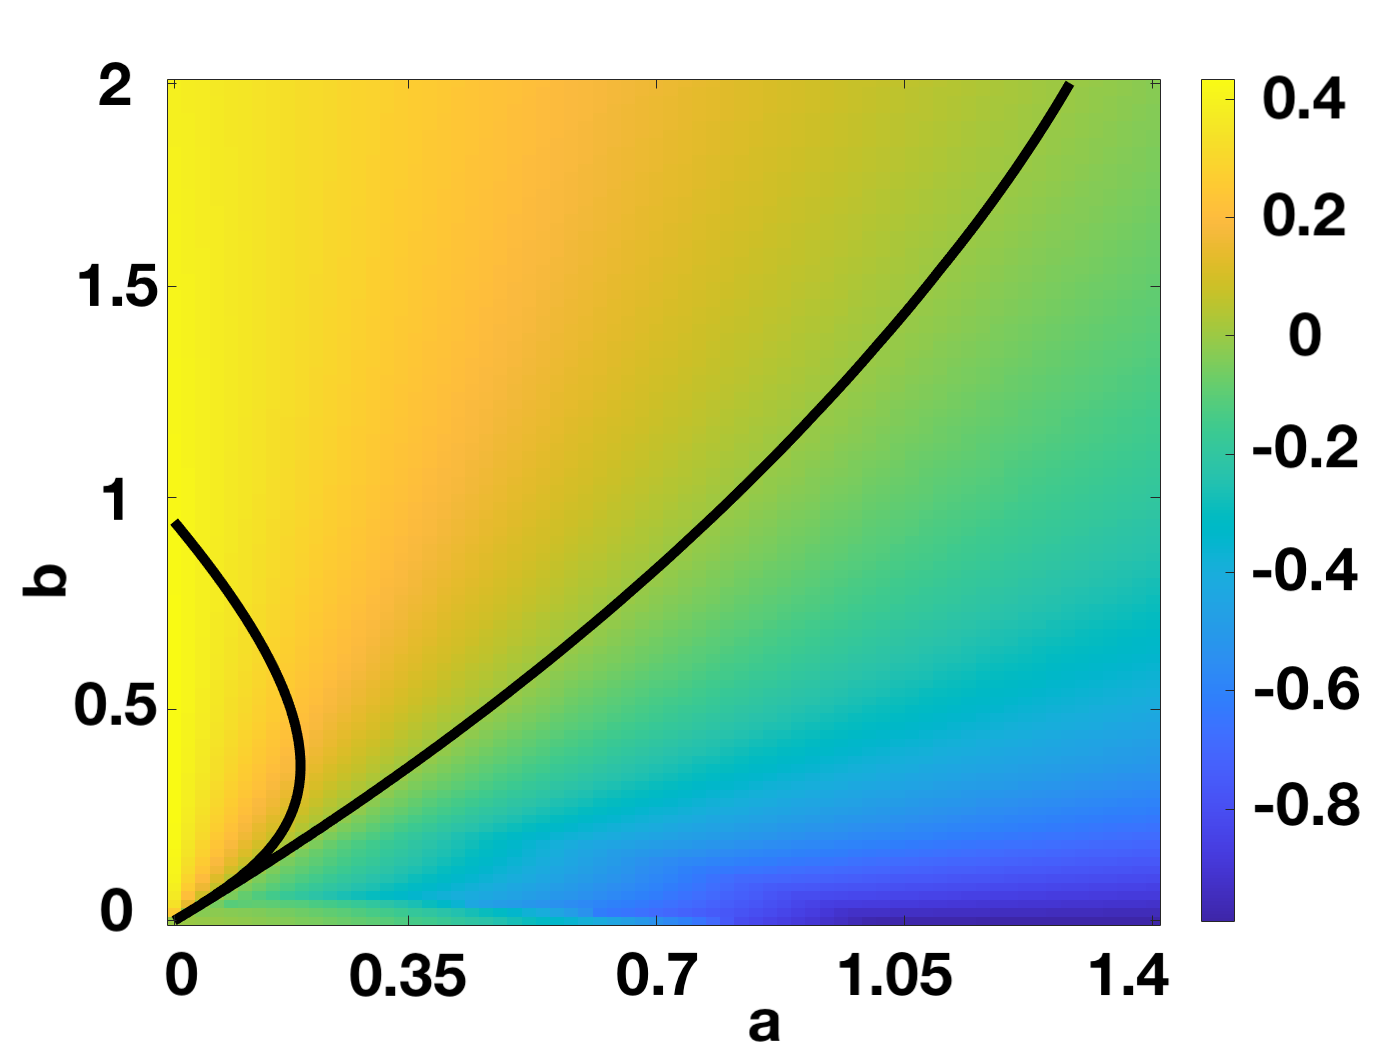
\includegraphics[width=7cm,height=4.75cm]{t1f1.png}
        \caption{$\tau=0.2$.}
        \label{}
    \end{subfigure}
    \hfill
    \begin{subfigure}[t]{0.45\textwidth}
        \centering
        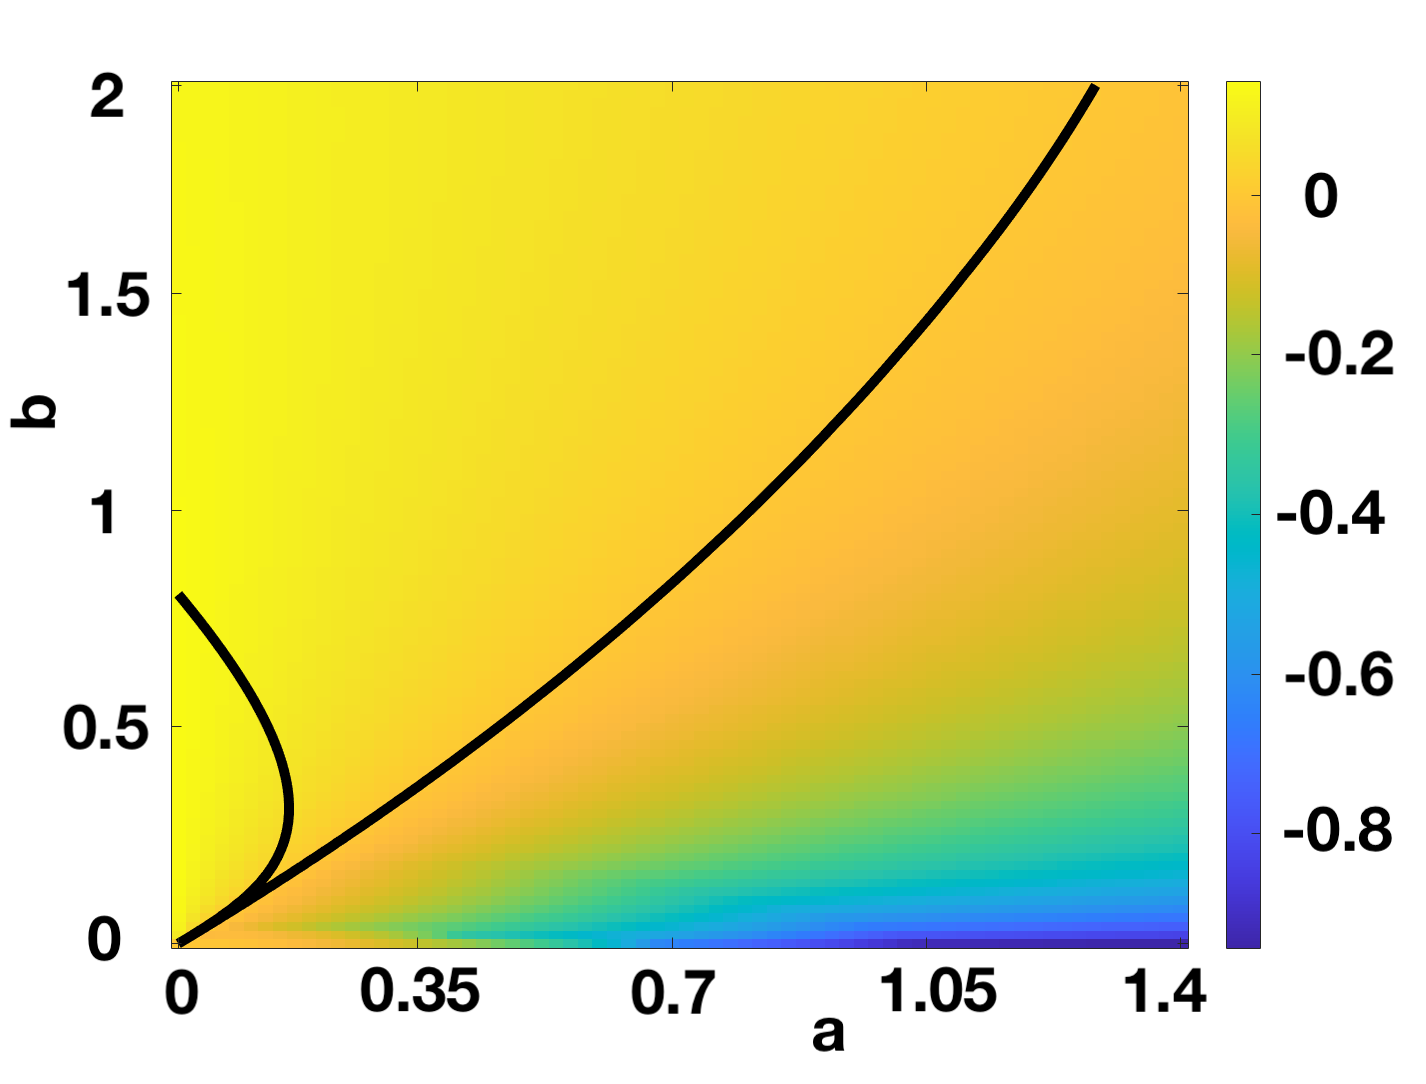
\includegraphics[width=7cm,height=4.75cm]{t2f1.png}
        \caption{$\tau=1$}
        \label{}
    \end{subfigure}
    \caption{Bifurcation diagrams produced by solving \eqref{characfix} (fixed delay characteristic equation) for $\tau=0.2,1$ and $\epsilon^2=0.001$, on a domain length $L^2=9/2$.}
    \label{fig:distheat1}
\end{figure}
\begin{figure}[H]
    \centering
    \begin{subfigure}[t]{0.45\textwidth}
        \centering
        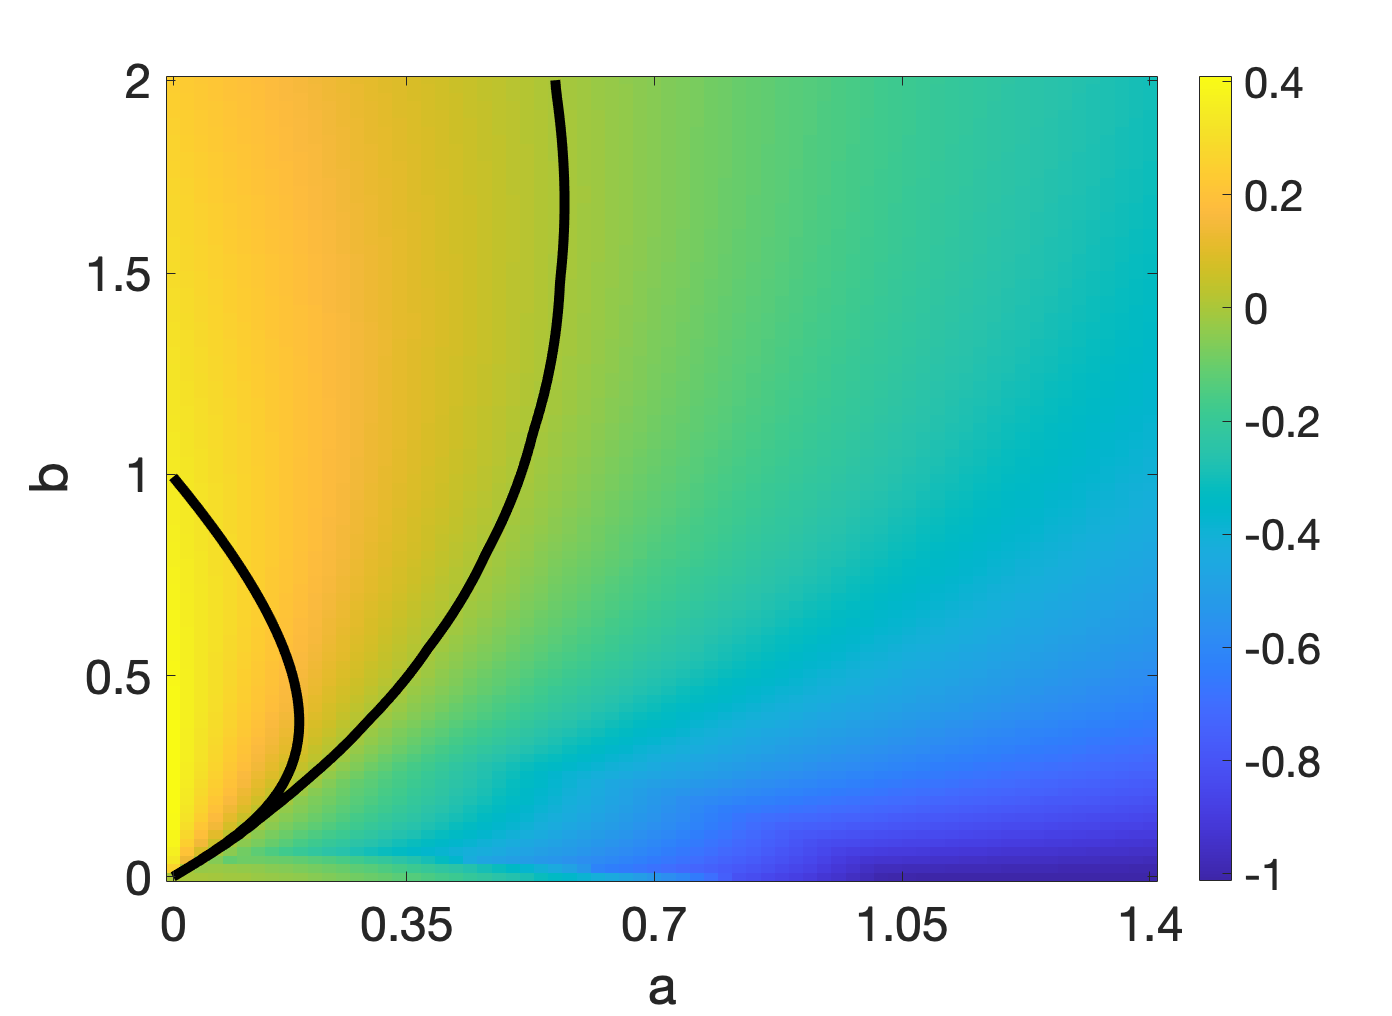
\includegraphics[width=7cm,height=4.75cm]{distbif3.png}
        \caption{$\tau=0.2$.}
        \label{}
    \end{subfigure}
    \hfill
    \begin{subfigure}[t]{0.45\textwidth}
        \centering
        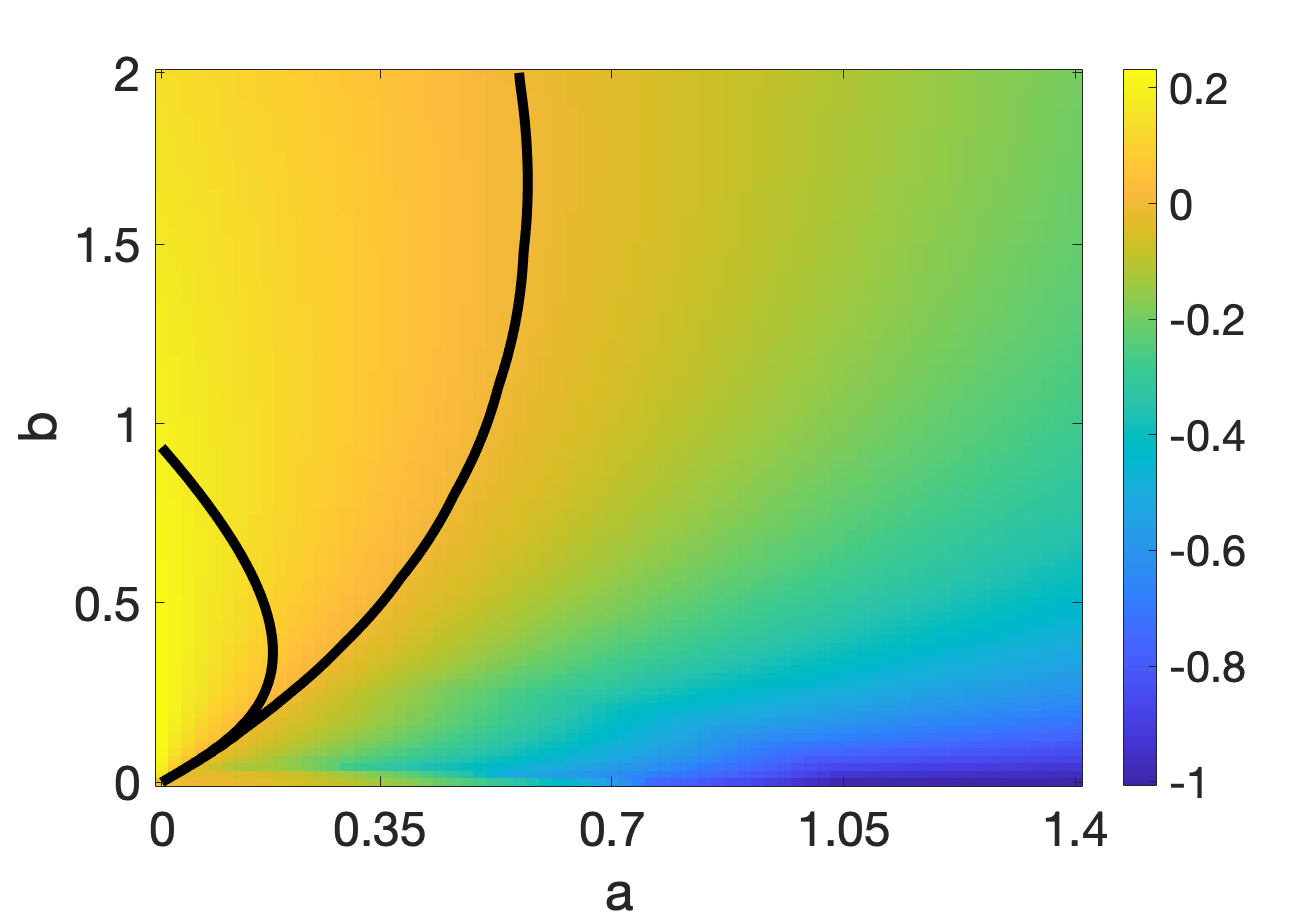
\includegraphics[width=7cm,height=4.75cm]{distbif4.png}
        \caption{$\tau=0.5$}
        \label{}
    \end{subfigure}
    \caption{Bifurcation diagrams produced by solving \eqref{characfix} (fixed delay characteristic equation) for $\tau=0.2,0.5$ and $\epsilon^2=0.01$, on a domain length $L^2=9/2$.}
    \label{fig:distheat2}
\end{figure}

\begin{figure}[H]
    \centering
    \begin{subfigure}[t]{0.45\textwidth}
        \centering
        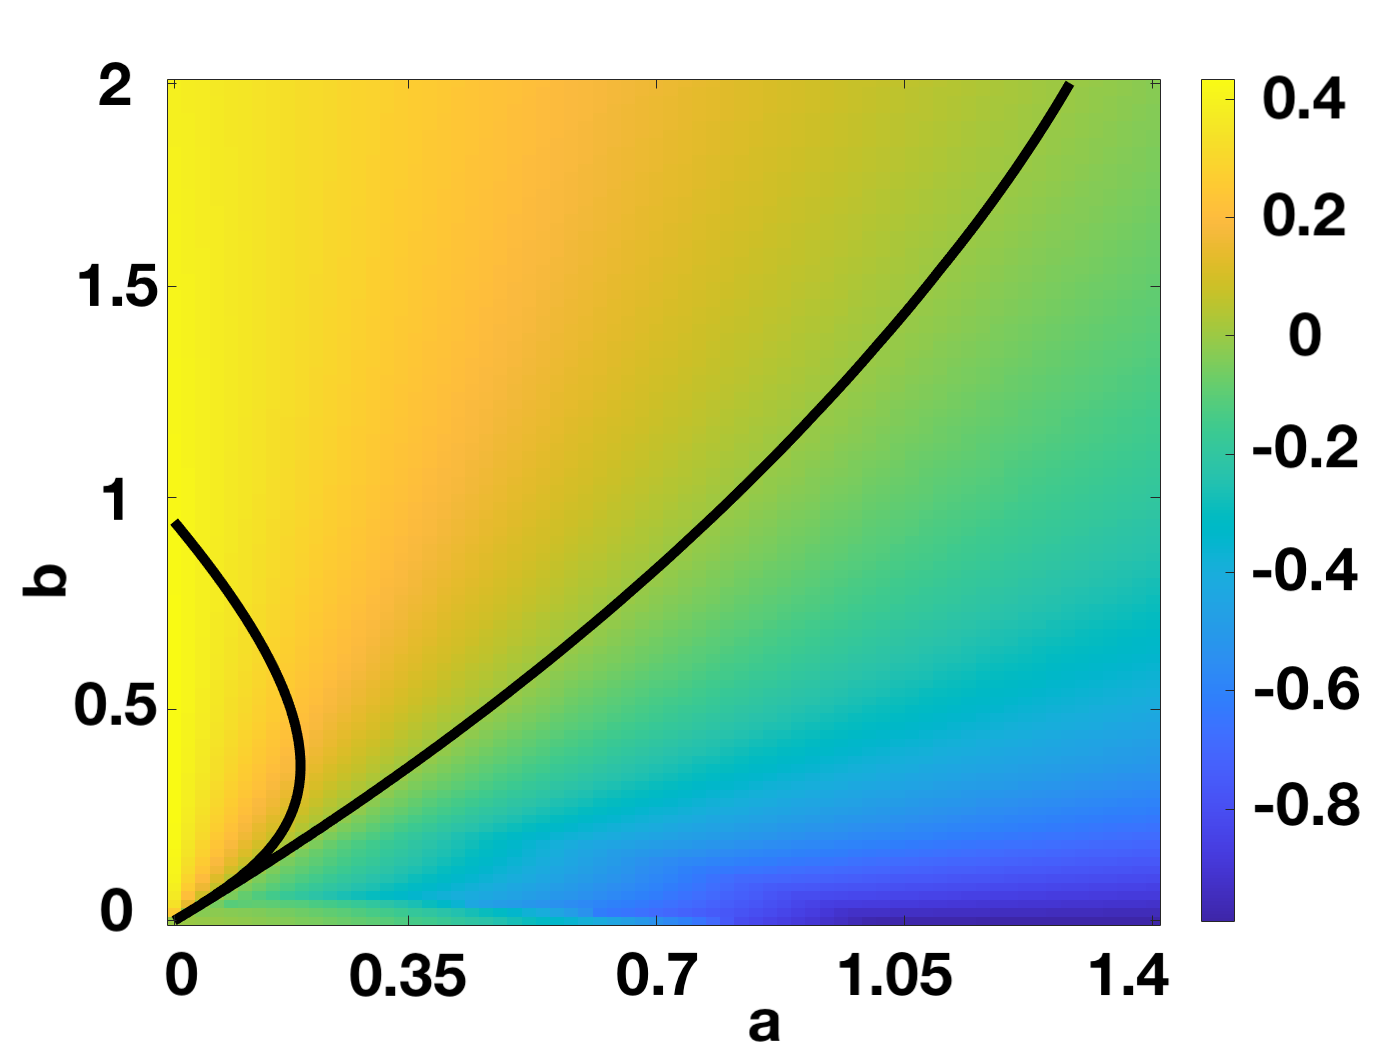
\includegraphics[width=7cm,height=4.75cm]{t1f1.png}
        \caption{Fixed delay case}
        \label{}
    \end{subfigure}
    \hfill
    \begin{subfigure}[t]{0.45\textwidth}
        \centering
        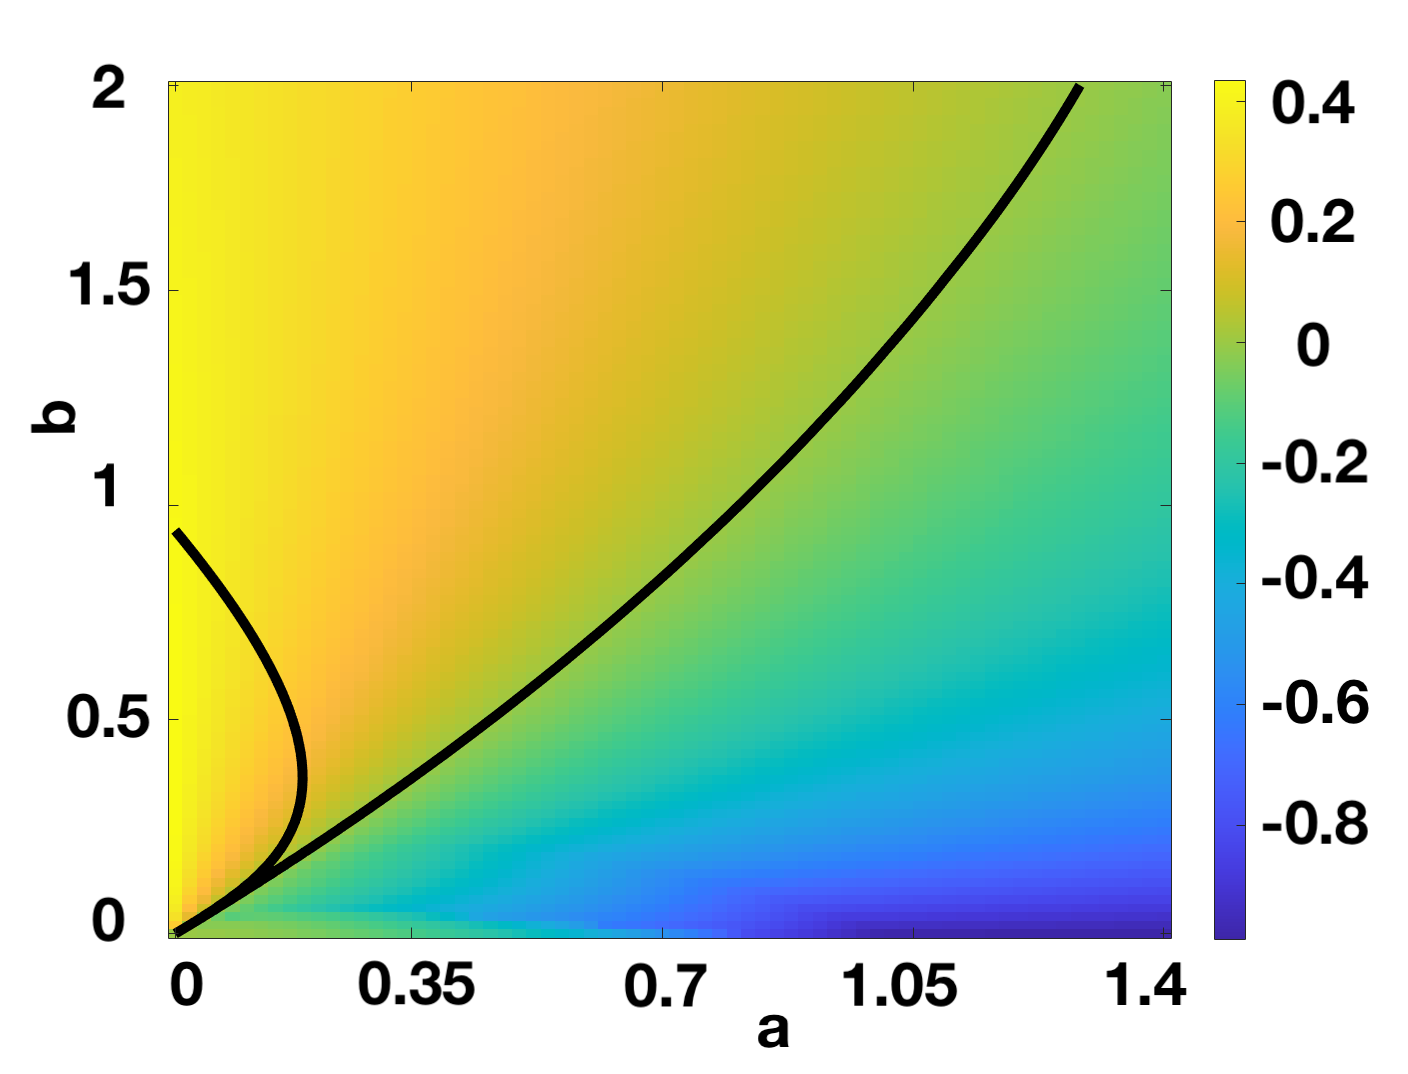
\includegraphics[width=7cm,height=4.75cm]{t1f2.png}
        \caption{$\sigma=\sigma_{\max}\times0.99$}
        \label{}
    \end{subfigure}
    \hfill
    \begin{subfigure}[t]{0.45\textwidth}
        \centering
        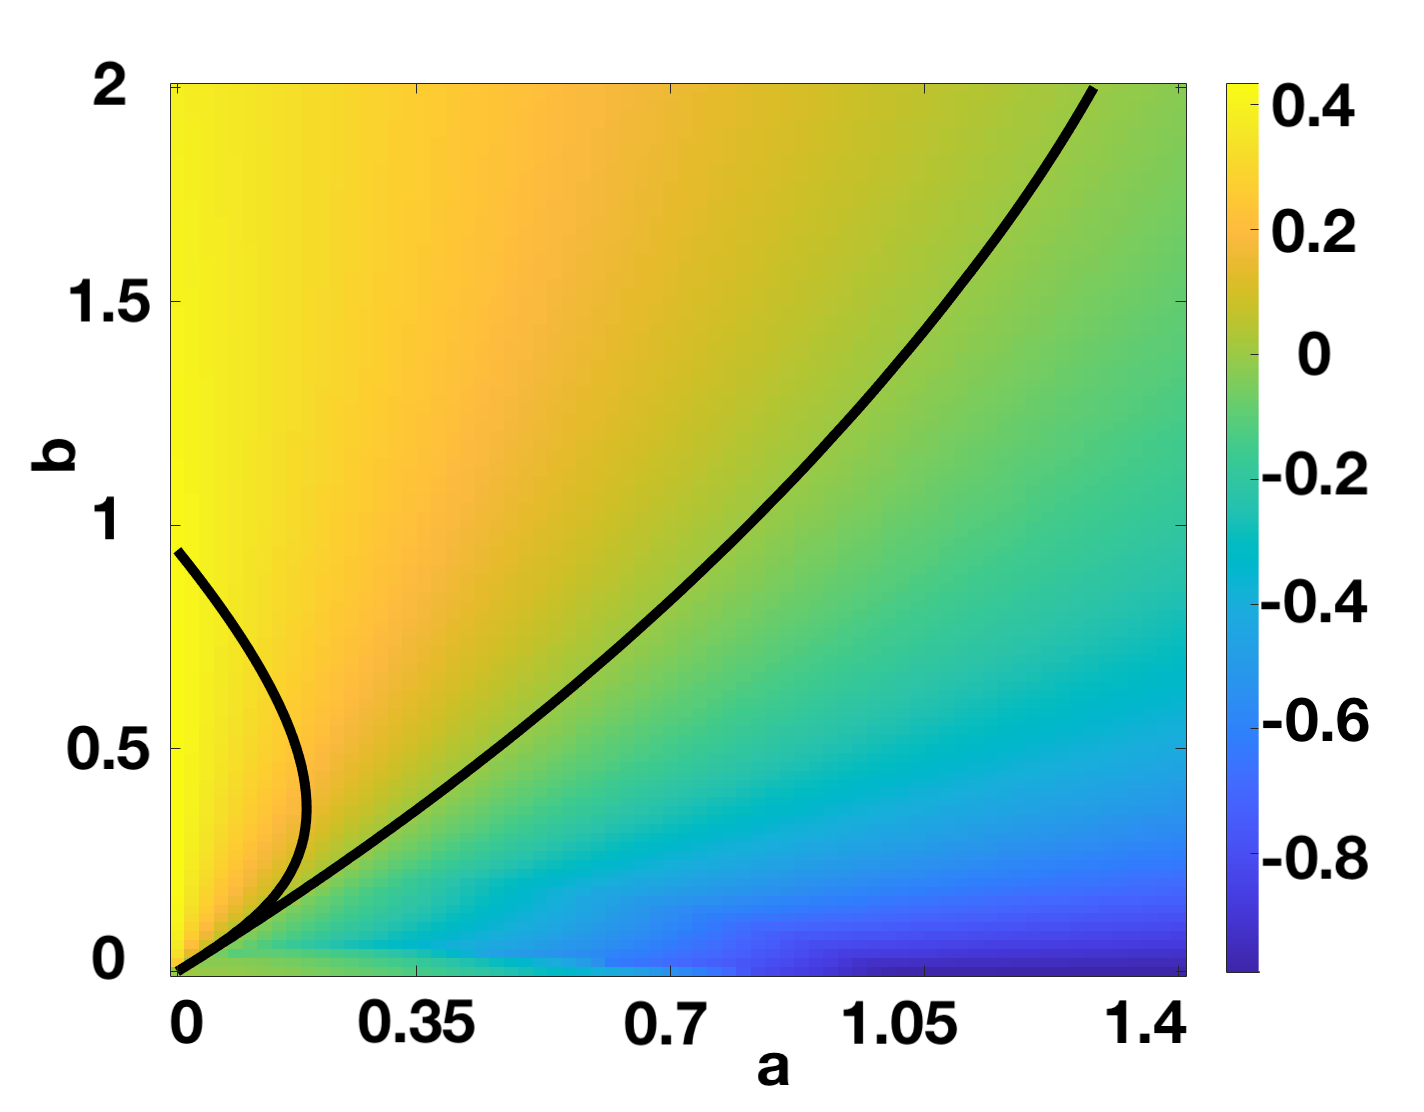
\includegraphics[width=7cm,height=4.75cm]{t1f3.png}
        \caption{$\sigma=\sigma_{\max}\times0.2$}
        \label{}
    \end{subfigure}
    \hfill
    \begin{subfigure}[t]{0.45\textwidth}
        \centering
        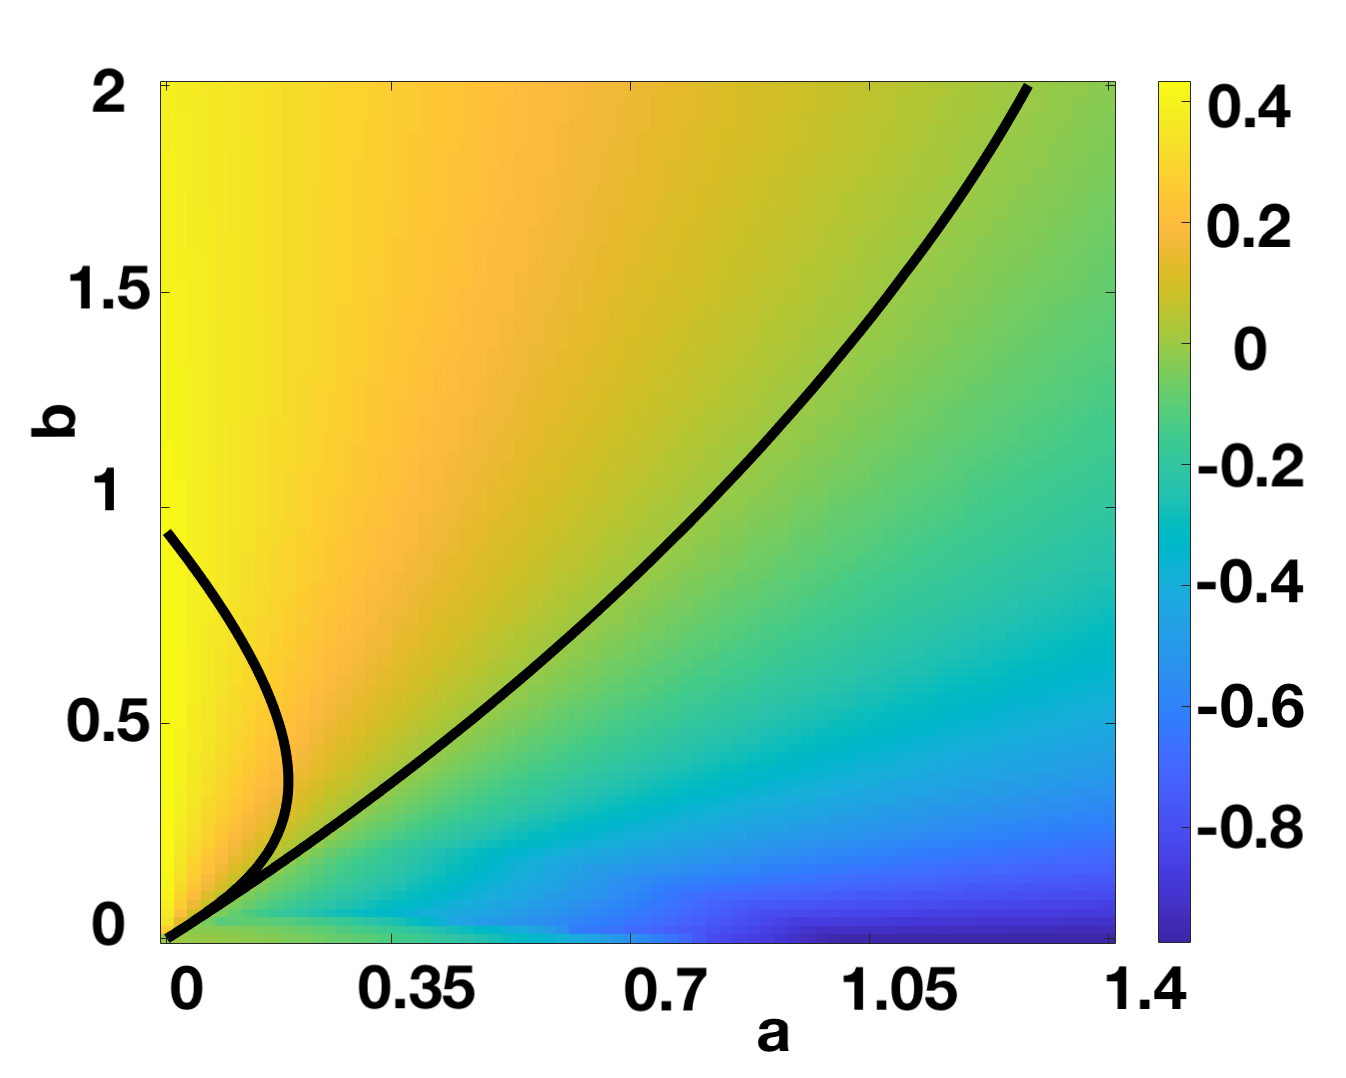
\includegraphics[width=7cm,height=4.75cm]{t1f4.png}
        \caption{$\sigma=\sigma_{\max}\times0.1$}
        \label{}
    \end{subfigure}
    \caption{Bifurcation diagrams for varying $\sigma$ for $\tau=0.2$ and $\epsilon^2=0.001$, on a domain length $L^2=9/2$.}
    \label{fig:distmap1}
\end{figure}

\begin{figure}[H]
    \centering
    \begin{subfigure}[t]{0.45\textwidth}
        \centering
        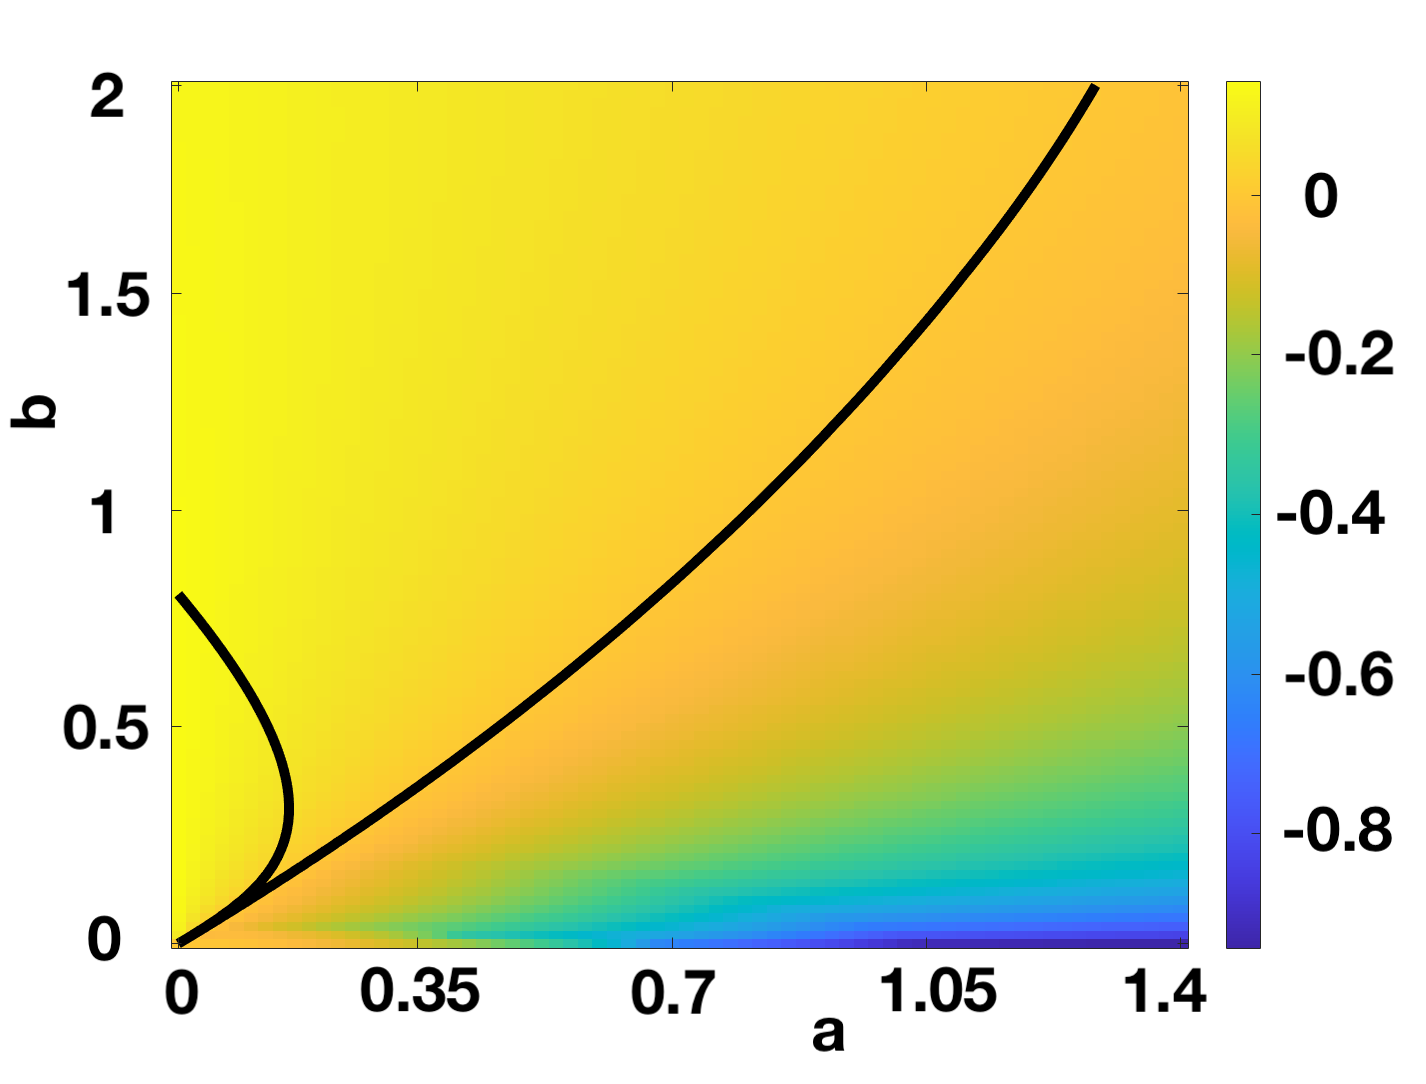
\includegraphics[width=7cm,height=4.75cm]{t2f1.png}
        \caption{Fixed delay case}
        \label{}
    \end{subfigure}
    \hfill
    \begin{subfigure}[t]{0.45\textwidth}
        \centering
        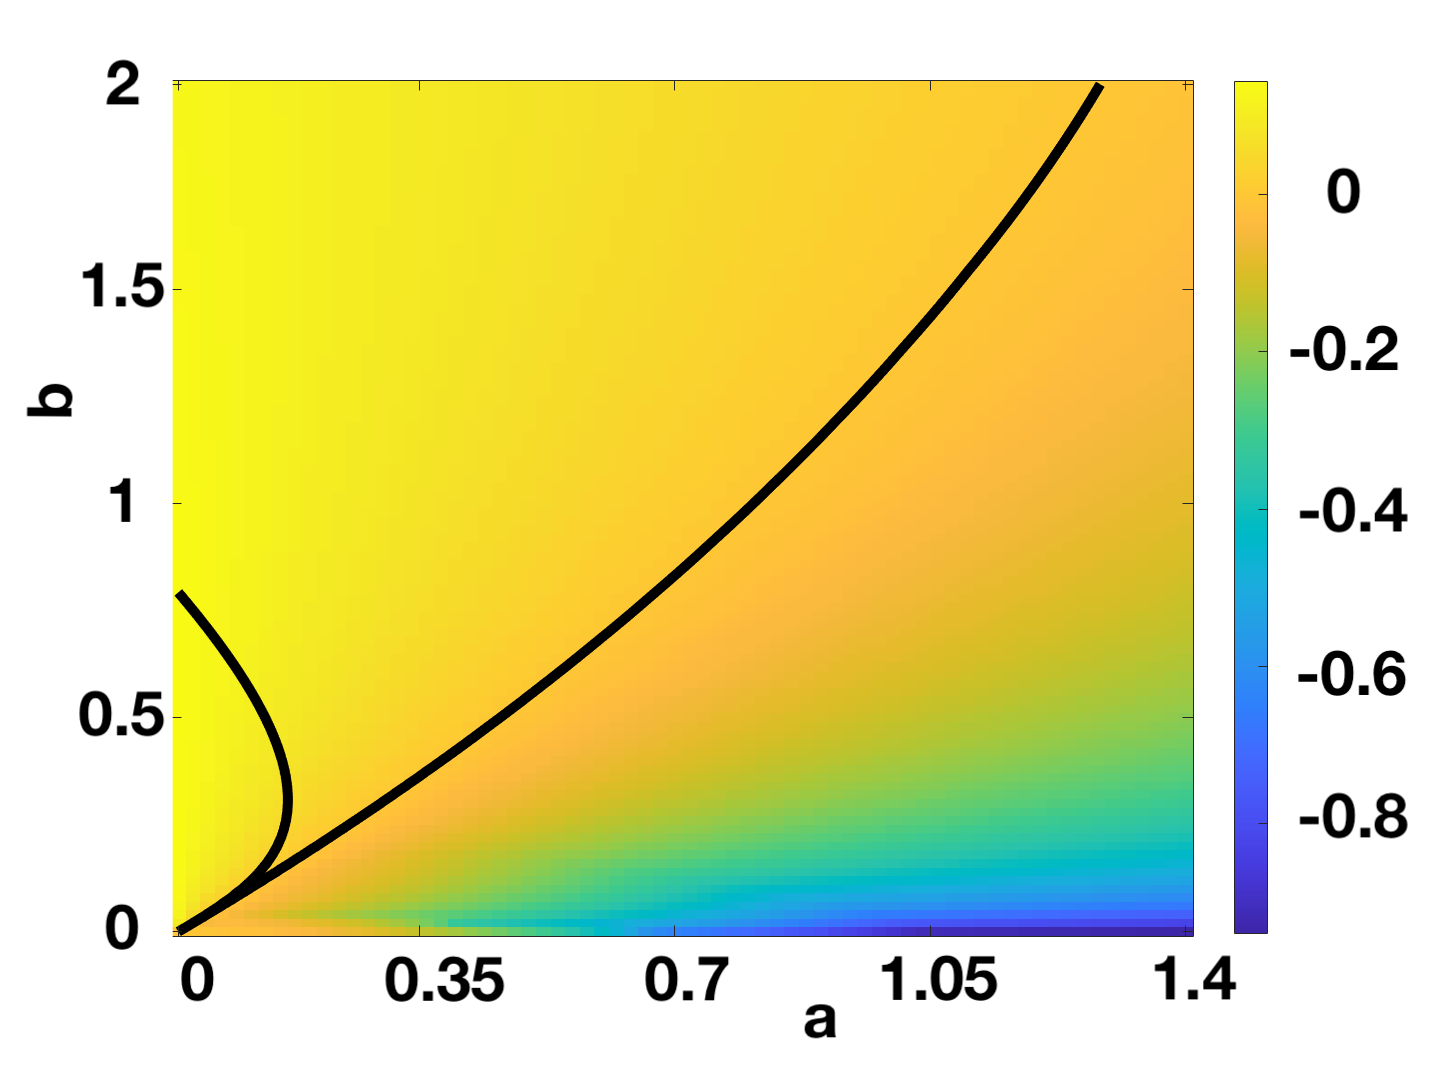
\includegraphics[width=7cm,height=4.75cm]{t2f2.png}
        \caption{$\sigma=\sigma_{\max}\times0.99$}
        \label{}
    \end{subfigure}
    \hfill
    \begin{subfigure}[t]{0.45\textwidth}
        \centering
        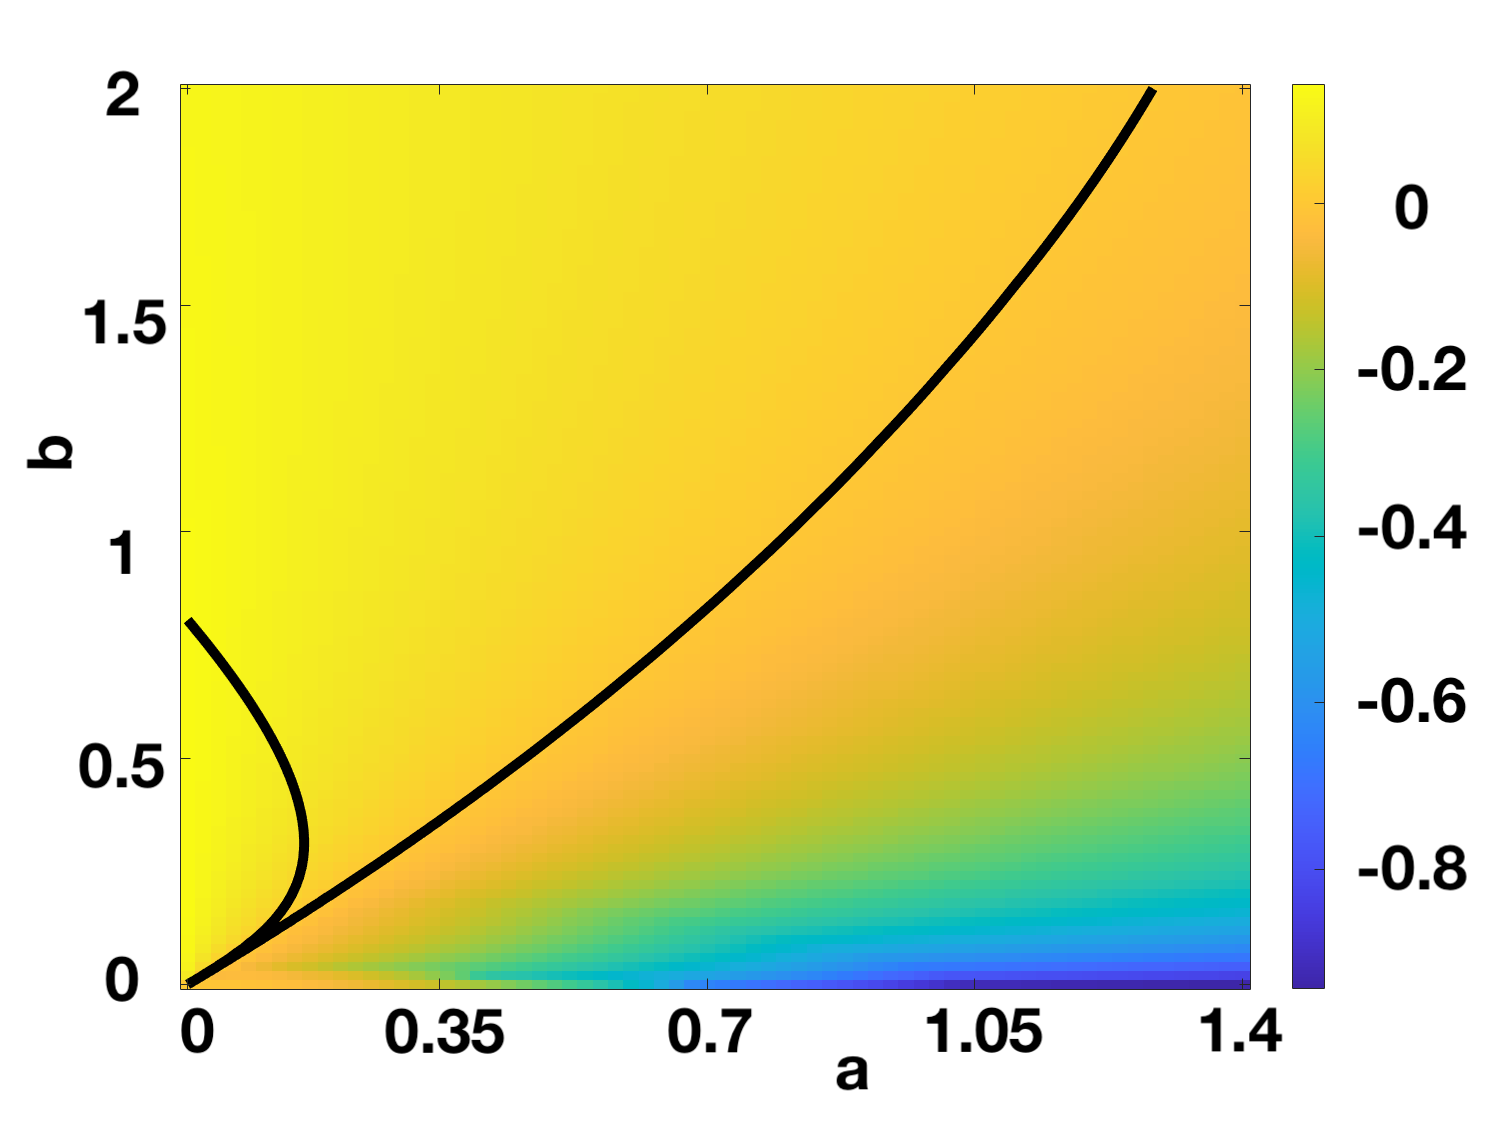
\includegraphics[width=7cm,height=4.75cm]{t2f3.png}
        \caption{$\sigma=\sigma_{\max}\times0.2$}
        \label{}
    \end{subfigure}
    \hfill
    \begin{subfigure}[t]{0.45\textwidth}
        \centering
        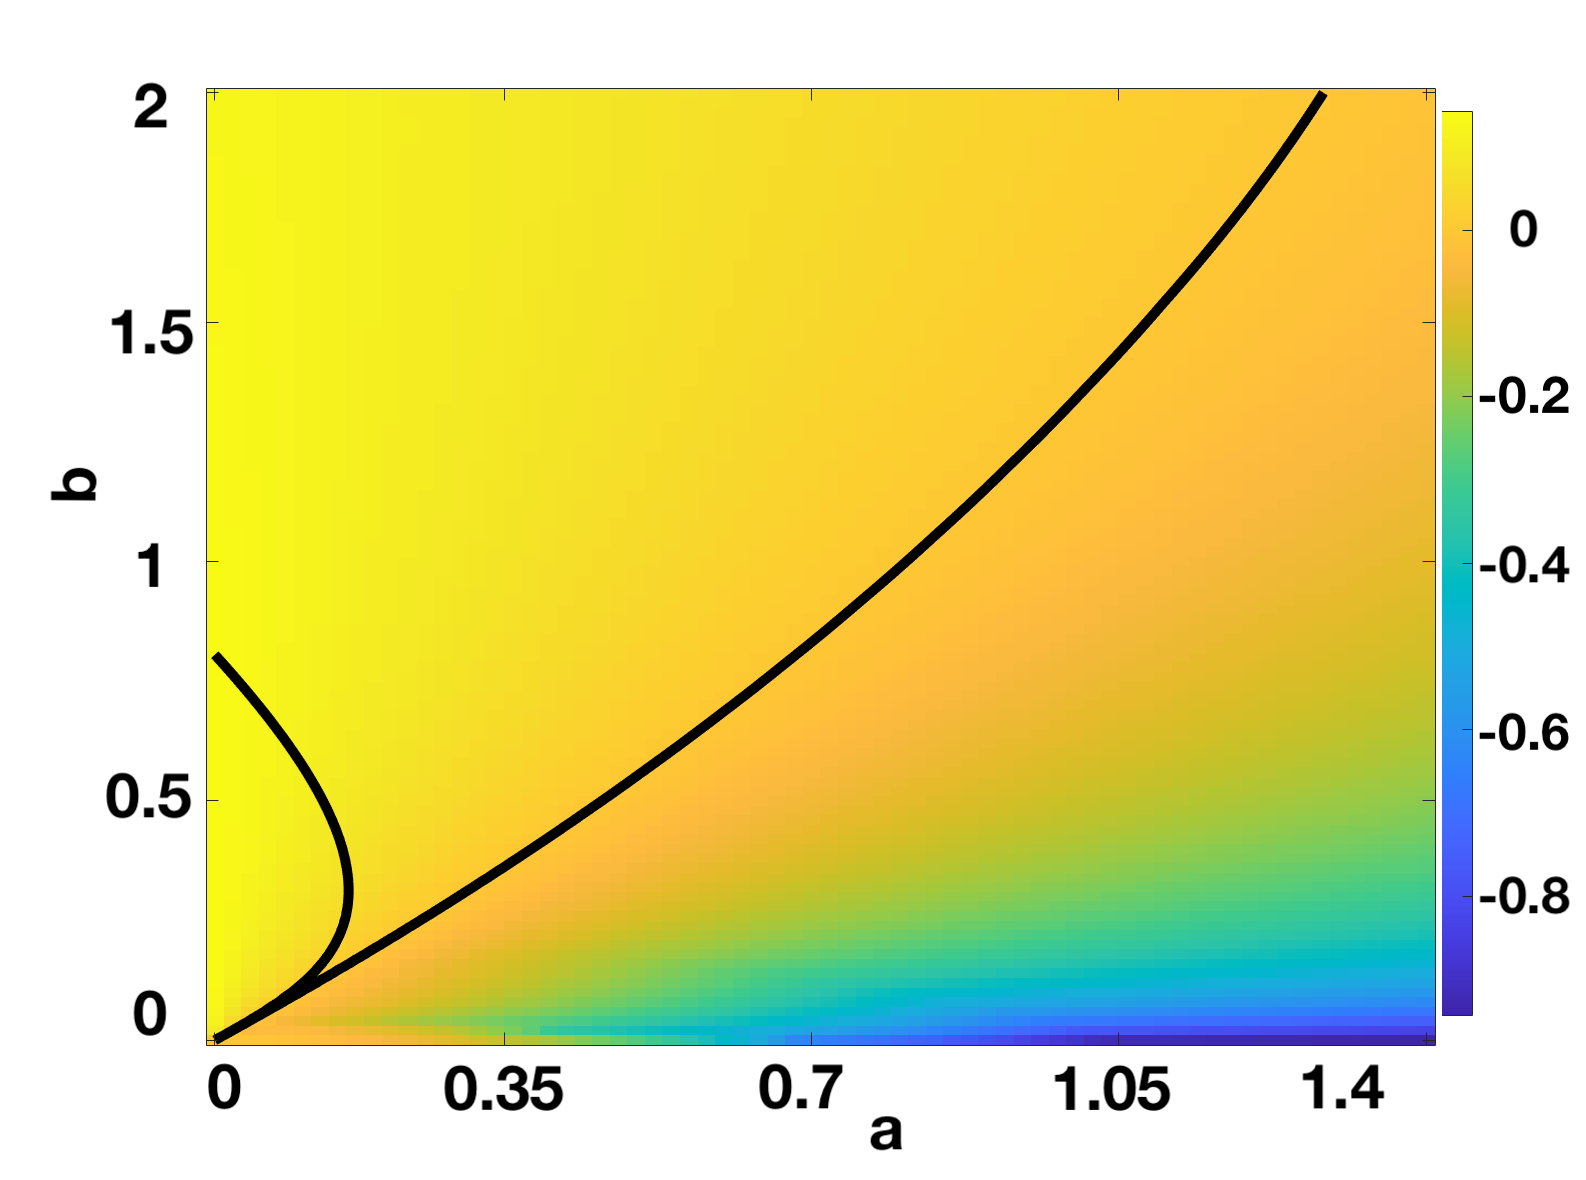
\includegraphics[width=7cm,height=4.75cm]{t2f4.png}
        \caption{$\sigma=\sigma_{\max}\times0.1$}
        \label{}
    \end{subfigure}
    \caption{Bifurcation diagrams for varying $\sigma$ for $\tau=1$ and $\epsilon^2=0.001$, on a domain length $L^2=9/2$.}
    \label{fig:distmap2}
\end{figure}

The linear theory from Figures \ref{fig:p2} and \ref{fig:p3} suggests that we have pattern formation for all $\tau\in[0,1]$ independent of the $\sigma$ used for $(a,b)=(0.1,0.9)$, but not for $(a,b)=(0.4,0.4)$. Figures \ref{fig:linapp1} and \ref{fig:linapp2} show similar results to those in \ref{fig:testdist1} and \ref{fig:testdist2}, but with $\tau=0.5$.

\begin{figure}[H]
    \centering
    \begin{subfigure}[t]{0.45\textwidth}
        \centering
        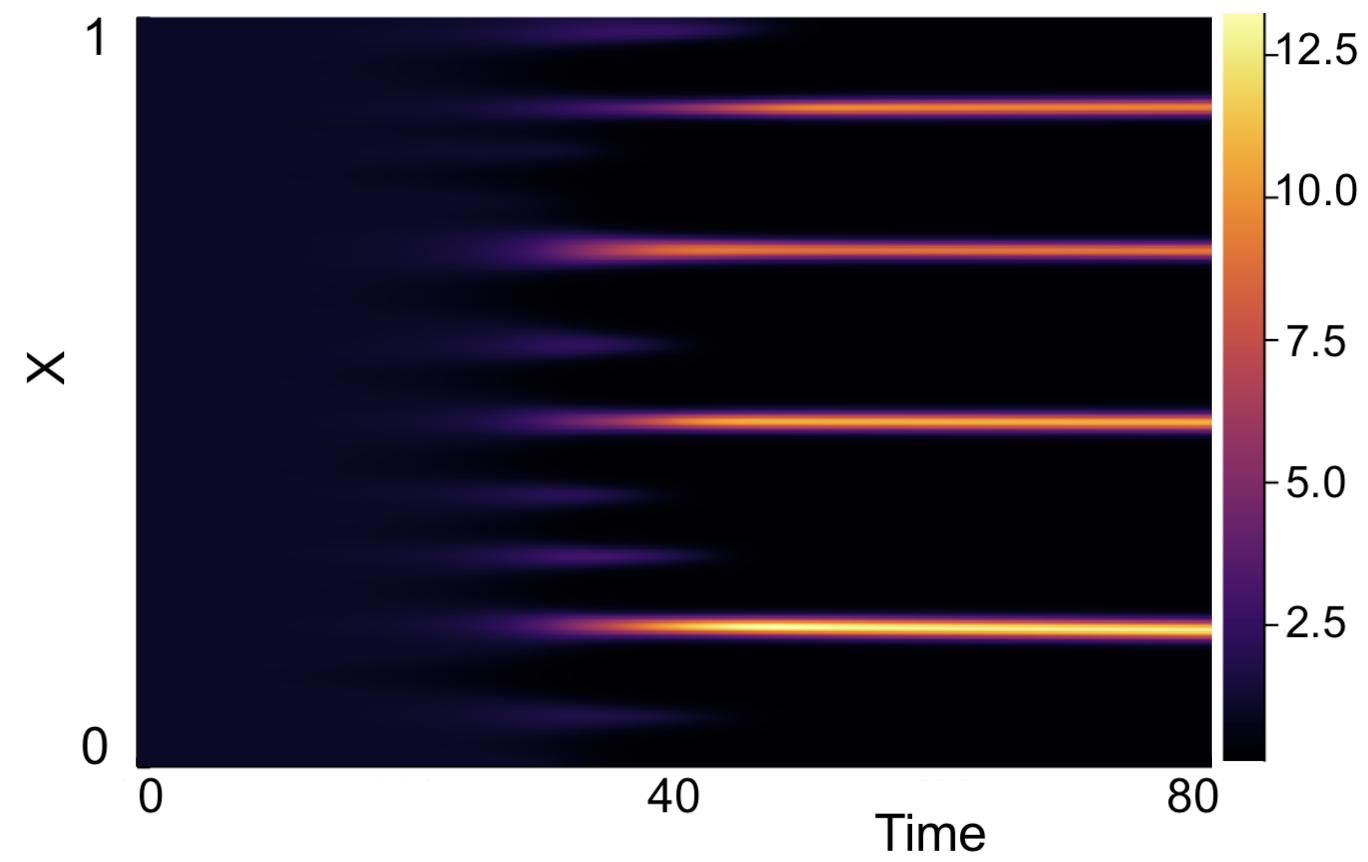
\includegraphics[width=7cm,height=5cm]{applin1.png}
        \caption{Numerical solution with $\tau=0.5$ and $\sigma=\sigma_{\max}\times0.99$.}
        \label{}
    \end{subfigure}
    \hfill
    \begin{subfigure}[t]{0.45\textwidth}
        \centering
        \includegraphics[width=7cm,height=5cm]{applin1.png}
        \caption{Numerical solution with $\tau=0.5$ and $\sigma=\sigma_{\max}\times0.1$.}
        \label{}
    \end{subfigure}
    \caption{Numerical solutions produced for $(a,b)=(0.1,0.9)$ with $\tau=0.5$ and $\sigma=\sigma_{\max}\times0.99, \sigma_{\max}\times0.1$. We use $L^2=9/2$ and $\epsilon^2=0.001$. Boundary conditions given by \eqref{neumannbc} and initial conditions by \eqref{firstic}. We see pattern formation, as predicted from linear theory.}
    \label{fig:linapp1}
\end{figure}

\begin{figure}[H]
    \centering
    \begin{subfigure}[t]{0.45\textwidth}
        \centering
        \includegraphics[width=7cm,height=5cm]{linapp2.png}
        \caption{Numerical solution with $\tau=0.5$ and $\sigma=\sigma_{\max}\times0.99$.}
        \label{}
    \end{subfigure}
    \hfill
    \begin{subfigure}[t]{0.45\textwidth}
        \centering
        \includegraphics[width=7cm,height=5cm]{linapp2.png}
        \caption{Numerical solution with $\tau=0.5$ and $\sigma=\sigma_{\max}\times0.1$.}
        \label{}
    \end{subfigure}
    \caption{Numerical solutions produced for $(a,b)=(0.4,0.4)$ with $\tau=0.5$ and $\sigma=\sigma_{\max}\times0.99, \sigma_{\max}\times0.1$. We use $L^2=9/2$ and $\epsilon^2=0.001$. Boundary conditions given by \eqref{neumannbc} and initial conditions by \eqref{firstic}. We see no pattern formation, as predicted from linear theory.}
    \label{fig:linapp2}
\end{figure}

Finally, we show futher numerical results, for the parameter set $(a,b)=(0.3,1.2)$, to support the conclusion that the onset of patterning, and the type of pattern we see, is independent of $\sigma$ used.

\begin{figure}[H]
   \centering
   \begin{subfigure}[t]{0.32\textwidth}
       \centering
       \includegraphics[width=5cm,height=4.5cm]{dist2t1sigmax.png}
       \caption{Fixed delay model given by \eqref{fixed2}.}
       \label{}
   \end{subfigure}
   \hfill
   \begin{subfigure}[t]{0.32\textwidth}
       \centering
       \includegraphics[width=5cm,height=4.5cm]{dist2t1sigmax.png}
       \caption{Distributed delay model, \eqref{symmod}, with $\sigma=\sigma_{\max}\times0.99$.}
       \label{}
   \end{subfigure}
   \hfill
   \begin{subfigure}[t]{0.32\textwidth}
       \centering
       \includegraphics[width=5cm,height=4.5cm]{dist2t1sigmax.png}
       \caption{Distributed delay model, \eqref{symmod}, with $\sigma=\sigma_{\max}\times0.1$.}
       \label{}
   \end{subfigure}
   \caption{Numerical simulations showing comparison of fixed delay case vs distributed delay case for $\tau=1$. Boundary conditions given by \eqref{neumannbc} and initial conditions by \eqref{firstic}. $(a,b)=(0.3,1.2)$, $\epsilon^2=0.001$, $L^2=9/2$.}
   \label{fig:distres3}
\end{figure}
\begin{figure}[H]
    \centering
    \begin{subfigure}[t]{0.32\textwidth}
        \centering
        \includegraphics[width=5cm,height=4.5cm]{dist2t16sigmax.png}
        \caption{Fixed delay model given by \eqref{fixed2}.}
        \label{}
    \end{subfigure}
    \hfill
    \begin{subfigure}[t]{0.32\textwidth}
        \centering
        \includegraphics[width=5cm,height=4.5cm]{dist2t16sigmax.png}
        \caption{Distributed delay model, \eqref{symmod}, with $\sigma=\sigma_{\max}\times0.99$.}
        \label{}
    \end{subfigure}
    \hfill
    \begin{subfigure}[t]{0.32\textwidth}
        \centering
        \includegraphics[width=5cm,height=4.5cm]{dist2t16sigmax.png}
        \caption{Distributed delay model, \eqref{symmod}, with $\sigma=\sigma_{\max}\times0.1$.}
        \label{}
    \end{subfigure}
    \caption{Numerical simulations showing comparison of fixed delay case vs distributed delay case for $\tau=16$. Boundary conditions given by \eqref{neumannbc} and initial conditions by \eqref{firstic}. $(a,b)=(0.3,1.2)$, $\epsilon^2=0.001$, $L^2=9/2$.}
    \label{fig:distres4}
\end{figure}

\subsection{An Asymmetric Distribution}

We present results here to verify that for larger $\tau$, the skewed distribution does not signficantly change the results seen compared to that of the fixed delay case. Figures here show the results for $\tau\in\{1,2,4,8\}$.

% tau = 1
\begin{figure}[H]
    \centering
    \begin{subfigure}[t]{0.45\textwidth}
        \centering
        \includegraphics[width=7cm,height=5cm]{skewdist1.png}
        \caption{pdfs of skewed truncated Gaussian distributions, with $\rho=-10,10$. Both pdfs have mean $\tau=1$.}
        \label{}
    \end{subfigure}
    \hfill
    \begin{subfigure}[t]{0.45\textwidth}
        \centering
        \includegraphics[width=7cm,height=5cm]{fixt1.png}
        \caption{Numerical simulation of fixed delay case with $\tau=1$.}
        \label{}
    \end{subfigure}
    \hfill
    \begin{subfigure}[t]{0.45\textwidth}
        \centering
        \includegraphics[width=7cm,height=5cm]{fixt1.png}
        \caption{Numerical simulation with skewed distribution of $\rho=-10$. Distribution parameters are $\mu=2.70(3 s.f.)$ and $\omega=0.891(3 s.f.)$.}
        \label{}
    \end{subfigure}
    \hfill
    \begin{subfigure}[t]{0.45\textwidth}
        \centering
        \includegraphics[width=7cm,height=5cm]{fixt1.png}
        \caption{Numerical simulation with skewed distribution of $\rho=10$. Distribution parameters are $\mu=1.59(3 s.f.)$ and $\omega=0.525(3 s.f.)$.}
        \label{}
    \end{subfigure}
    \caption{Numerical rsesults for $(a,b)=(0.1,0.9)$ with $\rho=-10,10$ and $\tau=2$. Parameters $\epsilon^2=0.001$ and $L^2=9/2$. Initial conditions given by \eqref{firstic} and boundary conditions by \eqref{neumannbc}.}
    \label{fig:linskew2}
\end{figure}

% tau = 2
\begin{figure}[H]
    \centering
    \begin{subfigure}[t]{0.45\textwidth}
        \centering
        \includegraphics[width=7cm,height=5cm]{distskew2.png}
        \caption{pdfs of skewed truncated Gaussian distributions, with $\rho=-10,10$. Both pdfs have mean $\tau=2$.}
        \label{}
    \end{subfigure}
    \hfill
    \begin{subfigure}[t]{0.45\textwidth}
        \centering
        \includegraphics[width=7cm,height=5cm]{fixt2.png}
        \caption{Numerical simulation of fixed delay case with $\tau=2.$}
        \label{}
    \end{subfigure}
    \hfill
    \begin{subfigure}[t]{0.45\textwidth}
        \centering
        \includegraphics[width=7cm,height=5cm]{fixt2.png}
        \caption{Numerical simulation with skewed distribution of $\rho=-10$. Distribution parameters are $\mu=2.70(3 s.f.)$ and $\omega=0.891(3 s.f.)$.}
        \label{}
    \end{subfigure}
    \hfill
    \begin{subfigure}[t]{0.45\textwidth}
        \centering
        \includegraphics[width=7cm,height=5cm]{skewt210.png}
        \caption{Numerical simulation with skewed distribution of $\rho=10$. Distribution parameters are $\mu=1.59(3 s.f.)$ and $\omega=0.525(3 s.f.)$.}
        \label{}
    \end{subfigure}
    \caption{Numerical rsesults for $(a,b)=(0.1,0.9)$ with $\rho=-10,10$ and $\tau=2$. Parameters $\epsilon^2=0.001$ and $L^2=9/2$. Initial conditions given by \eqref{firstic} and boundary conditions by \eqref{neumannbc}.}
    \label{fig:linskew2}
\end{figure}

% tau = 4
\begin{figure}[H]
    \centering
    \begin{subfigure}[t]{0.45\textwidth}
        \centering
        \includegraphics[width=7cm,height=5cm]{distt4.png}
        \caption{pdfs of skewed truncated Gaussian distributions, with $\rho=-10,10$. Both pdfs have mean $\tau=4$.}
        \label{}
    \end{subfigure}
    \hfill
    \begin{subfigure}[t]{0.45\textwidth}
        \centering
        \includegraphics[width=7cm,height=5cm]{fixt4.png}
        \caption{Numerical simulation of fixed delay case with $\tau=4.$}
        \label{}
    \end{subfigure}
    \hfill
    \begin{subfigure}[t]{0.45\textwidth}
        \centering
        \includegraphics[width=7cm,height=5cm]{fixt4.png}
        \caption{Numerical simulation with skewed distribution of $\rho=-10$. Distribution parameters are $\mu=5.41(3 s.f.)$ and $\omega=1.79(3 s.f.)$.}
        \label{}
    \end{subfigure}
    \hfill
    \begin{subfigure}[t]{0.45\textwidth}
        \centering
        \includegraphics[width=7cm,height=5cm]{fixt4.png}
        \caption{Numerical simulation with skewed distribution of $\rho=10$. Distribution parameters are $\mu=3.17(3 s.f.)$ and $\omega=1.05(3 s.f.)$.}
        \label{}
    \end{subfigure}
    \caption{Numerical rsesults for $(a,b)=(0.1,0.9)$ with $\rho=-10,10$ and $\tau=4$. Parameters $\epsilon^2=0.001$ and $L^2=9/2$. Initial conditions given by \eqref{firstic} and boundary conditions by \eqref{neumannbc}.}
    \label{fig:linskew4}
\end{figure}

% tau = 8
\begin{figure}[H]
    \centering
    \begin{subfigure}[t]{0.45\textwidth}
        \centering
        \includegraphics[width=7cm,height=5cm]{distskew8.png}
        \caption{pdfs of skewed truncated Gaussian distributions, with $\rho=-10,10$. Both pdfs have mean $\tau=8$.}
        \label{}
    \end{subfigure}
    \hfill
    \begin{subfigure}[t]{0.45\textwidth}
        \centering
        \includegraphics[width=7cm,height=5cm]{fixt8.png}
        \caption{Numerical simulation of fixed delay case with $\tau=8$.}
        \label{}
    \end{subfigure}
    \hfill
    \begin{subfigure}[t]{0.45\textwidth}
        \centering
        \includegraphics[width=7cm,height=5cm]{skewt8m10.png}
        \caption{Numerical simulation with skewed distribution of $\rho=-10$. Distribution parameters are $\mu=10.8(3 s.f.)$ and $\omega=3.58(3 s.f.)$.}
        \label{}
    \end{subfigure}
    \hfill
    \begin{subfigure}[t]{0.45\textwidth}
        \centering
        \includegraphics[width=7cm,height=5cm]{skewt810.png}
        \caption{Numerical simulation with skewed distribution of $\rho=10$. Distribution parameters are $\mu=6.34(3 s.f.)$ and $\omega=2.09(3 s.f.)$.}
        \label{}
    \end{subfigure}
    \caption{Numerical rsesults for $(a,b)=(0.1,0.9)$ with $\rho=-10,10$ and $\tau=8$. Parameters $\epsilon^2=0.001$ and $L^2=9/2$. Initial conditions given by \eqref{firstic} and boundary conditions by \eqref{neumannbc}.}
    \label{fig:linskew8}
\end{figure}
